\documentclass[11pt]{article}
\usepackage[margin=1in]{geometry}
\usepackage{amsmath,amssymb,amsthm,booktabs,array}
\usepackage{tikz,pgfplots}
\usepackage[hidelinks]{hyperref}
\pgfplotsset{compat=1.18}
\newtheorem{theorem}{Theorem}[section]
\newtheorem{lemma}[theorem]{Lemma}
\newtheorem{proposition}[theorem]{Proposition}
\newtheorem{corollary}[theorem]{Corollary}
\theoremstyle{remark}
\newtheorem{remark}[theorem]{Remark}
\numberwithin{equation}{section}
\newcommand{\E}{\mathbb E}
\newcommand{\Pp}{\mathbb P}
\newcommand{\Fbar}{\overline F}
\newcommand{\Rplus}{\mathbb R_+}
\newcommand{\ind}{\mathbf 1}
\newcommand{\OPT}{\operatorname{OPT}}
\newcommand{\MF}{\operatorname{MF}}
\newcommand{\GP}{\operatorname{G}}
\newcommand{\PS}{\operatorname{PS}}
\newcommand{\RV}{\operatorname{RV}}
\newcommand{\eps}{\varepsilon}
\newcolumntype{L}[1]{>{\raggedright\arraybackslash}p{#1}}
\DeclareMathOperator{\supp}{supp}

\title{Finite Load Advice: Mathematical Argument}
\author{Haoyi Zhang \and Huaijin Ran}
\date{}
\hypersetup{
  pdftitle={Finite Load Advice: Mathematical Argument},
  pdfauthor={Haoyi Zhang and Huaijin Ran},
  pdfkeywords={queueing, online scheduling, finite advice, maximum flow time, regular variation, processor sharing}
}
\begin{document}
\maketitle
This self-contained argument accompanies the finite scheduling artifact.
The results are mathematical derivations, not machine-checked theorems.
The stationary and asymptotic claims are not established by the finite tests.
\section{Two guarantees for the same policy}\label{sec:intro}
A queueing policy can protect the largest response time on each finite input or protect the asymptotic response-time tail of a typical arrival. These are different requirements. A finite-input guarantee compares schedules on the same released jobs. A stationary tail guarantee compares probabilities under a specified arrival and service law. Neither comparison can be substituted for the other, even when both use response time as their underlying quantity.

Heavy-tailed service times make the distinction concrete. On every finite unit-speed single-server input, first-come, first-served (FCFS) minimizes the maximum response time. Yet a long job can delay many smaller arrivals under FCFS. Processor sharing (PS) removes this exclusive blocking but has no finite maximum-flow competitive factor. Classical queueing analyses instead ask for waiting- or sojourn-time asymptotics under a fixed stochastic model. Regular variation and subexponentiality provide the language for those asymptotics~\cite{cohen1973,bingham1987,abate1994,abate1997,foss2013}; busy-period and processor-sharing results identify how one large service requirement propagates through a queue~\cite{zwart2001,zwartboxma2000,guillemin2004,borst2006,mandjes2006}. The question here is not whether heavy-tail protection is possible without advice. It is what deterministic maximum-flow guarantee can accompany that protection, and how one finite environment message changes the choice of that guarantee.

The distinction matters beyond notation. Size-aware and age-aware disciplines can drastically change a response distribution even though every work-conserving discipline has the same workload path. SRPT, foreground-background, Gittins, and their variants have been analyzed through exact transforms, sample-path comparisons, index policies, or rank functions~\cite{schrage1966,nunez2002,nuyenswierman2008,nuyenssmart2008,nuyenszwart2006,aalto2009,gittins2011,scully2018soap}. General sufficient conditions now cover broad heavy-tailed policy classes, including policies that do not observe job sizes~\cite{scully2020characterizing,scullyvankreveld2024}. These results establish that job-size-order tails are achievable. They do not attach a finite adversarial maximum-flow certificate to the same policy.

We consider a message sent once for an entire queue environment. A public collection contains $M$ policies. Each has its own worst-case competitive factor on arbitrary finite inputs. An oracle, knowing the load or even the entire service law, chooses one policy from the collection. The message contains no processing times of individual jobs and no information about the future realized arrival sequence. We ask how closely the selected factor can track the smallest factor compatible with a stationary heavy-tail guarantee.

The load is the decisive parameter. Write
\begin{equation}\label{eq:theta-intro}
 \theta(\rho)=\frac{1}{1-\rho},\qquad 0<\rho<1.
\end{equation}
We prove that $\theta(\rho)$ is a strict boundary: factors below it are incompatible with job-size-order tails, while every factor above it is attainable. The statement at equality is separate and remains open in this analysis. Thus a finite message is useful on a bounded envelope of $\theta$, but no fixed finite collection of finite-competitive policies covers loads arbitrarily close to one.

\subsection{The closest tail-scheduling boundaries}
The most direct predecessor is the question posed by Wierman and Zwart~\cite{wierman2012}. Their GI/GI/1 framework considers work-conserving, nonanticipating, nonlearning policies and permits a job's size to become available at or after arrival. Their weak-tail comparison asks whether one policy can remain within a finite multiplicative tail scale of the best policy over broad light- and heavy-tailed distribution classes. The resulting impossibility concerns simultaneous distributional robustness. Our theorem does not negate or evade that result by renaming its information. We restrict the law to a regularly varying finite-mean class, allow one global law-dependent selection before the queue runs, and impose a second objective that is absent from their comparison: an unconditional maximum-flow ratio on every finite input. The lower bound here is therefore a capacity statement about that joint objective, not a universal tail-competitiveness theorem.

Nair, Wierman, and Zwart~\cite{nair2010} give the closest load-indexed policy family. Limited processor sharing serves at most a configured number of jobs simultaneously and uses the load to trade heavy- and light-tailed behavior. Their analysis obtains tail exponents and a weak robustness conclusion for the stochastic response distribution. It does not show that the configured policy has a finite maximum-flow ratio on every arrival sequence, and it does not lower-bound the number of global messages needed to approximate a load-dependent adversarial factor. Simply relabeling an LPS parameter as advice would consequently leave both halves of our joint statement unproved.

A later line of work characterizes tail-optimal scheduling more directly. Scully et al.~\cite{scully2020characterizing} give policy-level sufficient conditions for heavy-tailed response-time optimality using the SOAP framework~\cite{scully2018soap}; related analyses cover SMART, Gittins, RMLF, and limited-preemption or noisy-rank variants~\cite{nuyenssmart2008,scully2018bubbles,scully2020simple,scully2020gittins,scully2021gittins,scullyvankreveld2024}. The positive theorem below is compatible with the broad message of this literature---a sufficiently protected large job need not force an integrated response tail---but its proof uses a different decomposition. An oldest-job reserve proves a finite-prefix certificate, while only the residual capacity is compared with PS. The construction is not a SOAP rank rule, and we do not claim that the SOAP conditions imply its deterministic guarantee.

Tail order must also be separated from a leading asymptotic constant. For regularly varying sizes, classical PS results can identify exact or near-exact asymptotics under additional assumptions~\cite{zwartboxma2000,borst2006,guillemin2004}; for other disciplines, comparison and ordering results give different stochastic guarantees~\cite{shanthikumar1987,boxmadenisov2011}. Yu and Scully~\cite{yu2024} make the weak-versus-strong distinction explicit and construct strongly tail-optimal policies in a light-tailed M/G/1. Nudge and related policies provide stochastic improvements within an FCFS-oriented light-tail setting~\cite{grosof2021,vanhoudt2022,charlet2024}. We prove only an order upper bound in the regularly varying setting. The physical inequality $T\geq B$ makes that order optimal, but the constants obtained from conditional moments are not claimed to be sharp.

Table~\ref{tab:closest-work} records the theorem-level differences that are essential for the present claims. The ``information'' column refers to what selects or drives the online rule, not what an analyst knows after a run.

\begin{table}[t]
\centering
\small
\caption{Closest theorem families and the precise separation from the present joint objective. ``RV'' means regularly varying.}\label{tab:closest-work}
\begin{tabular}{@{}L{0.13\textwidth}L{0.15\textwidth}L{0.24\textwidth}L{0.37\textwidth}@{}}
\toprule
Work & Information & Principal guarantee & Difference needed here\\
\midrule
Wierman--Zwart~\cite{wierman2012} & No learned law; arrived sizes may be known & Weak tail competitiveness across broad light/heavy classes & No global load message and no finite-input maximum-flow certificate; their impossibility and ours quantify over different objectives\\
Nair--Wierman--Zwart~\cite{nair2010} & Load-configured LPS parameter & Stochastic tail exponent and weak robustness & No exact maximum-flow factor and no finite-message covering lower bound\\
Scully et al.~\cite{scully2020characterizing} & SOAP rank, possibly size blind & Sufficient conditions for heavy-tail order optimality & Characterizes tail behavior, not simultaneous adversarial maximum flow\\
Yu--Scully~\cite{yu2024} & Distribution-aware boost rule & Strong light-tail optimality; heavy-tail appendix & Different tail class and benchmark; no environment-message complexity\\
Advice complexity~\cite{bocken2009,emek2011,boyar2016} & Oracle tape derived from a realized online input & Bits needed to improve a competitive ratio & Our message identifies an environment before its random input is realized and cannot encode that realization\\
Predictions\newline\cite{lykouris2018,purohit2018,mitzenmacher2022} & Predictions with an error-dependent guarantee & Consistency and robustness tradeoff & No predictor or error metric is estimated here; every selected code has an unconditional finite-input certificate\\
This paper & One finite global environment message & RV tail order and exact finite-input maximum-flow factor for the same policy & Strict factor boundary and optimal logarithmic covering on a bounded load envelope\\
\bottomrule
\end{tabular}
\end{table}

\subsection{A reservation policy and a capacity obstruction}
The positive construction has a simple rate rule. With $N$ active jobs, reserve rate $\delta\in(0,1)$ for the oldest job and distribute the remaining rate $1-\delta$ equally among all active jobs. Consequently, the oldest job receives $\delta+(1-\delta)/N$, while each other job receives $(1-\delta)/N$. The rule uses arrival order and the active set, not job sizes. We call it \emph{$\delta$-guarded sharing} and write it as $\GP_\delta$.

The oldest-job reservation protects every arrival prefix, not only one distinguished job. As long as some job released by time $a$ is unfinished, the oldest active job belongs to that prefix. The prefix therefore receives at least $\delta$ units of service per unit time. Its remaining work at $a$ is at most the offline optimal maximum flow time. This gives a competitive factor $1/\delta$, which is the exact worst-case factor of the policy.

The remaining service behaves differently. Each job receives at least its share under an ordinary PS queue of speed $1-\delta$. If $\rho<1-\delta$, that slower comparison queue is stable. A permanent-customer construction bounds its size-conditional response moments using only its load, not higher service-time moments. Integrating the conditional bound against a regularly varying service distribution proves a job-size-order response tail. Choosing $\delta=1/C$ gives the sufficient condition $C>\theta(\rho)$.

The converse does not assume that a policy uses a reservation. Start a busy cycle with one job of size $b$. A factor $C$ requires that job to complete within approximately $Cb$ on a long typical future arrival prefix. If $C<\theta(\rho)$, serving it this quickly consumes more than the spare capacity of that prefix. Choose a finite truncation of the service distribution whose load is already greater than $1-1/C$. Then an amount of order $b$ of bounded-job work remains unfinished after the large job has completed. Since each of these jobs has bounded size, an order-$b$ number of arrivals have long responses. Counting them in disjoint busy cycles converts the probability of a size-$b$ root into an integrated-tail lower bound. The truncation step is what avoids an unjustified inference from unfinished work to a number of unfinished jobs.

\subsection{The theorem ladder}
Let $\Fbar(x)=\Pp(B>x)=x^{-\alpha}L(x)$, where $\alpha>1$ and $L$ is slowly varying. Let $T$ denote the response time of a typical stationary arrival. The precise policy class and advice model appear in Section~\ref{sec:model}. The main statements are as follows.

\begin{theorem}[Strict load boundary]\label{thm:boundary-intro}
Fix an M/G/1 environment of unit-speed load $\rho\in(0,1)$ and service tail in $\RV(-\alpha)$, $\alpha>1$.
If an eligible policy has a finite-input maximum-flow competitive factor $C<\theta(\rho)$, then
\begin{equation}\label{eq:lower-intro}
 \liminf_{x\to\infty}\frac{\Pp(T>x)}{x\Fbar(x)}>0.
\end{equation}
For every $C>\theta(\rho)$, the nonclairvoyant policy $\GP_{1/C}$ has worst-case factor exactly $C$ and satisfies
\begin{equation}\label{eq:upper-intro}
 \limsup_{x\to\infty}\frac{\Pp(T>x)}{\Fbar(x)}<\infty.
\end{equation}
\end{theorem}

The necessary condition is policy independent within the stated causal and regenerative class. It still applies if the policy knows sizes of jobs that have already arrived. The sufficient condition uses less information. This asymmetry strengthens the lower bound; it is not a comparison that grants the proposed algorithm stronger information than its adversary.

For the information consequence, fix a public envelope $1<u<v<\infty$ for $\theta$. Let $c_m$ be the exact finite-input competitive factor of policy $m$. A valid selection rule supplies job-size-order tails for every admissible environment in the envelope. Its inflation is the worst selected value of $c_m/\theta$. Infima are taken over public collections and valid selection rules.

\begin{theorem}[Finite-message infimum]\label{thm:advice-intro}
With at most $M\geq1$ advised policies, the infimum inflation on $\theta\in[u,v]$ is
\begin{equation}\label{eq:advice-intro}
 \Gamma_M^*(u,v)=\left(\frac vu\right)^{1/M}.
\end{equation}
For a fixed-length budget of $b$ bits, one can take $M=2^b$. Finite rational codebooks approach the infimum with any prescribed positive slack. The theorem does not assert attainment at zero slack.
\end{theorem}

The covering step is elementary but its interpretation is not. A single competitive factor $c$ can serve only loads with $\theta\leq c$, and inflation at most $\Gamma$ additionally requires $\theta\geq c/\Gamma$. On a logarithmic scale, one policy covers an interval of length at most $\log\Gamma$. The scheduling content is the necessity of $c\geq\theta$ for every eligible policy, together with realizability above that boundary by the same policy that has the claimed adversarial guarantee.

A finite message is not a finite public description. Our rational construction stores $M$ boundaries and $M$ guards. These public quantities must be encoded and evaluated as well. We account for their bit lengths separately rather than hiding an arbitrary-precision real number in a transmitted policy index.

\subsection{Information models and why their quantifiers differ}
Classical competitive analysis fixes an input sequence and compares an online schedule with an offline optimum~\cite{borodin1998,albers2003}. Nonclairvoyant flow-time scheduling shows how job-size uncertainty and speed augmentation change achievable guarantees~\cite{kalyan1997,kalyan2000,kalyan2003,becchetti2004}. Standard scheduling texts emphasize that maximum flow, total flow, lateness, and stochastic sojourn time are distinct objectives~\cite{pinedo2016,lenstra2020}. Our benchmark belongs to this adversarial tradition, but the message does not: it is chosen from the queue law before the realized input exists.

The advice-complexity literature normally lets an oracle inspect the entire realized request sequence and write bits to a tape~\cite{bocken2009,hromkovic2010,emek2011,komm2011,boyar2016}. Under that model, $b$ bits can select among $2^b$ behaviors tailored to the particular sequence. Here $b$ bits select among $2^b$ fixed queueing policies using only the environment. All arrival and service randomness remains unknown when the message is sent. This restriction is why a one-dimensional covering argument is meaningful: the oracle can identify a load bin but cannot encode which future busy cycle will contain a large root.

Learning-augmented algorithms make another tradeoff. A prediction may be attached to a request or instance, and performance degrades as an error measure grows~\cite{lykouris2018,purohit2018,mitzenmacher2022}. Recent scheduling work combines learned information with competitive fairness or stochastic signals~\cite{li2025,cosson2026}. Those models motivate preserving a worst-case fallback, but neither their observations nor their objectives equal the global-message model here. We do not train a predictor, estimate a load interval from samples, or claim a guarantee as a function of prediction error. Incorrect advice preserves only the unconditional maximum-flow certificate; it may cross the tail boundary.

\subsection{Scope of the contribution}
The proof has three independent layers. First, workload gives a policy-independent maximum-flow benchmark and the oldest-job reserve turns it into an exact certificate. Second, a slower-PS domination and a permanent-customer moment calculation establish the positive tail result without assuming a finite moment of order above $\alpha$. Third, a regenerative large-root argument yields a policy-independent integrated-tail obstruction. Only after those layers meet do logarithmic covering and rational encoding translate the boundary into an advice theorem.

Several nearby results remain outside the claim. Heavy-traffic guarantees for blind policies~\cite{bansal2018}, multiserver SRPT and Gittins analyses~\cite{grosof2018,scully2020gittins,hong2024}, load-balancing guardrails~\cite{grosof2019}, and fairness-oriented or priority-control models~\cite{friedman2003,fajardo2015,fajardo2017,gavish1977} address different limits or objectives. Empirical heavy-tail observations motivate why response tails matter~\cite{crovella1996,harcholbalter2003}, but this paper makes no trace or deployment claim. The equality $C=\theta(\rho)$, exact leading tail constants, non-Poisson arrival extensions, and parallel-server analogues are left open rather than inferred from the finite checks.

The next section fixes the quantifiers and the workload benchmark. Section~\ref{sec:reservation} proves the deterministic reservation results. Sections~\ref{sec:tail} and~\ref{sec:obstruction} establish the two sides of the load boundary. Section~\ref{sec:advice} derives the finite-message theorem and finite encodings. Section~\ref{sec:boundaries} treats wrong messages, unbounded message lengths, and an explicitly faster server. Exact finite consequences and the limits of the result complete the argument.

\section{Inputs, information, and the workload benchmark}\label{sec:model}
\subsection{Finite scheduling inputs}
A finite input is a collection $I=\{(a_i,b_i):1\leq i\leq n\}$ with release times $a_i\geq0$ and processing requirements $b_i>0$. Jobs have fixed identifiers that break ties in release time. Their numerical values convey no information: a policy is invariant under relabeling that preserves this tie order, and no external arrival counter is supplied across an empty-state reset. At time $t$, a schedule assigns nonnegative measurable rates $s_i(t)$ to released unfinished jobs. A unit-speed schedule obeys
\begin{equation}\label{eq:capacity}
 \sum_i s_i(t)\leq1
\end{equation}
for almost every $t$. A job completes at the first time $d_i$ when its accumulated service reaches $b_i$. It receives no service before release or after completion. Preemption and simultaneous sharing carry no cost.

The response time, also called flow time, is $d_i-a_i$. Define
\begin{equation}\label{eq:maxflow}
 \MF_A(I)=\max_i(d_i^A-a_i),\qquad
 \OPT(I)=\inf_S\max_i(d_i^S-a_i),
\end{equation}
where the infimum allows any feasible unit-speed offline schedule, including a size-aware schedule that idles. Empty inputs have both values zero. A policy is $C$-competitive if $\MF_A(I)\leq C\OPT(I)$ for every nonempty finite input. We use no additive constant. Its exact competitive factor is
\begin{equation}\label{eq:exact-factor}
 c(A)=\sup_{I\ne\varnothing}\frac{\MF_A(I)}{\OPT(I)}.
\end{equation}
A finite supremum is itself a valid factor, whether or not any input attains it.

This is the maximum of individual response times, not their sum or average. The offline schedule knows the whole finite input. The online policy does not. In particular, a factor for the total flow objective would not establish any inequality in~\eqref{eq:maxflow}.

\subsection{The admissible policy class}
An eligible policy is deterministic, work conserving, and causal. Causality has a prefix-consistency requirement: two inputs whose released-job histories agree through time $h$ induce the same service before $h$. An eventual job count, input-ending time, or future-trace-dependent initialization is not supplied to the policy. If the policy uses current job sizes, those sizes are part of the revealed history; unreleased jobs are not.

The policy is invariant under a common shift of all release times. At an empty queue, it resets to a fixed empty state determined by its selected code. Consequently, busy cycles under a fixed stochastic environment are regenerative. The code itself is not discarded at a reset. Within a busy cycle the policy may maintain history and use all information available under its observation model. No claim is made for a policy that carries a learned distribution estimate across empty cycles without satisfying an appropriate uniform starting-state guarantee.

These conditions have distinct roles. Work conservation gives a common workload and busy-cycle decomposition. Prefix consistency transfers a guarantee on a finite prefix to the same prefix of an infinite arrival stream. Empty-state regeneration turns cycle rewards into stationary arrival probabilities. The positive construction satisfies all three directly. For the lower bound, we allow current-size information, making its admissible class at least as informative as the nonclairvoyant class used in the construction.

\subsection{A global finite message}
Fix public numbers $1<u<v<\infty$ and a collection $\mathcal A=(A_1,\ldots,A_M)$ of eligible policies with $c(A_m)<\infty$. The collection, including all numerical parameters, is fixed before choosing an environment. A message selects one member for the entire queue. The oracle may know the load and service distribution, but not the realized future arrivals or job sizes. The online policy has no additional law-dependent parameter other than its public definition and the selected code.

For each code, the finite-input guarantee is unconditional: it must hold for every finite input, even when the stochastic environment was misclassified. This requirement differs from a guarantee only on traces typical under the oracle's claimed law. It also differs from encoding a future finite schedule into a single unconstrained real-valued parameter.

An environment selection rule is valid if its selected policy has the required stationary tail for every environment in the public envelope. Its performance is
\begin{equation}\label{eq:inflation-def}
 \Gamma(\mathcal A,\phi)
   =\sup_{(\lambda,F)}
      \frac{c(A_{\phi(\lambda,F)})}{\theta(\lambda\E B)},
 \qquad \theta(\rho)=\frac1{1-\rho},
\end{equation}
where the supremum ranges over the regularly varying environments defined below with $\theta\in[u,v]$. Infima of this quantity concern the worst-case competitive factor selected by the message. They are not statistical sample complexities for estimating $\rho$ from observations.

At most $b$ fixed-length bits give at most $2^b$ messages. The public codebook may be much larger than $b$ bits: it contains the policies, interval endpoints, and service parameters. Section~\ref{sec:encoding} constructs finite rational parameters and accounts for this separate description cost.

\subsection{The stochastic environment and its tail objective}
Arrivals form a Poisson process of rate $\lambda>0$. Their positive service requirements are independent and identically distributed as $B$, independent of the arrival process. Put
\begin{equation}\label{eq:load}
 \mu=\E B<\infty,\qquad \rho=\lambda\mu\in(0,1).
\end{equation}
We assume
\begin{equation}\label{eq:rv}
 \Fbar(x)=\Pp(B>x)=x^{-\alpha}L(x),\qquad \alpha>1,
\end{equation}
where $L(cx)/L(x)\to1$ for every fixed $c>0$. No density is required. The distribution may have atoms, and its variance may be infinite. A statement conditional on $B=b$ is interpreted through a regular conditional distribution and therefore only needs to hold for $F$-almost every $b$.

The response time $T_A$ is that of a typical stationary arrival, rather than a root conditioned to start a busy period. For eligible policies, the common workload regeneration gives this arrival distribution through cycle rewards. We call
\begin{equation}\label{eq:tail-order}
 \limsup_{x\to\infty}\frac{\Pp(T_A>x)}{\Fbar(x)}<\infty
\end{equation}
a \emph{job-size-order tail guarantee}. Since $T_A\geq B$ at unit speed, a smaller order than $\Fbar$ is impossible. The guarantee allows a multiplicative constant depending on the fixed environment. It does not imply a uniform threshold in $x$ over all regularly varying laws.

For a fixed load, regular variation also gives
\begin{equation}\label{eq:scale-equivalence}
 \Fbar((1-\rho)x)\sim(1-\rho)^{-\alpha}\Fbar(x).
\end{equation}
Thus either tail scale can be used for a finite-order bound. We use the scaled denominator when presenting load-uniform bounds on asymptotic constants. We do not infer that the leading constant in this scaled comparison equals one.

\subsection{Assumption-to-proof map and nearby relaxations}\label{sec:assumption-map}
The assumptions above are not a single indivisible queueing convention.  Each enters at a particular proof interface.  Making those interfaces explicit prevents two common overextensions: importing a stationary queueing result into the finite-input benchmark without checking its information model, and treating a proof for Poisson input as if only the mean rate mattered.  Standard point-process and queueing references supply the Palm, Poisson, and regenerative background used at these interfaces~\cite{kingman1993,baccelli2003,bremaud2020,harcholbalter2013}.

\begin{table}[t]
\centering
\small
\caption{Where the model assumptions enter.  The last column states a possible proof obligation, not a theorem claimed here.}\label{tab:assumption-map}
\begin{tabular}{@{}L{0.19\textwidth}L{0.36\textwidth}L{0.35\textwidth}@{}}
\toprule
Assumption & Use in the present proof & What a relaxation would require\\
\midrule
Unit speed and preemption & Make unfinished work the common prefix certificate and let guarded sharing allocate rates continuously & A new benchmark under setup costs, indivisible service, or nonpreemptive blocking\\
Work conservation & Makes the workload path and busy-period endpoints independent of service order & Explicit control of intentional idling and of cycles that can be merged by the policy\\
Prefix consistency & Transfers the finite-input competitive deadline to the identical prefix of the infinite stochastic queue & A guarantee uniform over terminal horizons or an observation model that reveals the horizon\\
Empty-state reset & Makes policy state regenerative jointly with the workload & A stationary-state or Markov-renewal argument uniform over inherited internal states\\
Poisson arrivals & Give an independent future after the busy-cycle root, Poisson arrival sampling, and the stationary PS construction & Renewal/Palm replacements plus a new invariant-law or domination proof\\
IID positive sizes, independent of arrivals & Give the compound-Poisson laws of large numbers and isolate the root mark from future work & Mixing or dependence conditions strong enough for uniform fluid events and cycle rewards\\
Regular variation with $\alpha>1$ & Converts conditional moments to $\Fbar$ order and converts the large-root window to $x\Fbar(x)$ & Tail-class-specific integral estimates; finite-mean stability alone does not supply them\\
\bottomrule
\end{tabular}
\end{table}

The deterministic half of the argument uses neither Poisson arrivals nor regular variation.  Lemma~\ref{lem:workload}, the exact guarded-sharing factor, and the rational codebook are statements about arbitrary finite release sequences.  Stochastic assumptions first enter when the same rate rule is placed in stationarity.  This separation is useful operationally: a wrong environment message can destroy the tail guarantee while leaving the finite-input certificate intact.

The Poisson assumption is used in three distinguishable ways.  First, after a root arrival to an empty queue, the future marked process is independent of that root's service requirement.  Second, a typical arrival sees the stationary prearrival state; this is the PASTA step~\cite{wolff1982}.  Third, the processor-sharing comparison admits the residual product form verified in Lemma~\ref{lem:ps-invariant}.  A renewal input with the same rate would still have a strong law, but it would not automatically retain the latter two properties.  Consequently, replacing Poisson input is not a notational change: one would need the appropriate Palm arrival law and a replacement for the permanent-customer invariant distribution.

The empty-state reset is similarly stronger than stability of the workload alone.  All work-conserving disciplines share the workload process, but a policy can carry an internal estimate or random seed from one busy period to the next.  The reset rules out such cross-cycle memory so that delayed-job rewards form identically distributed regenerative cycles.  A stateful learner could be admitted only after proving a stationary initialization and a reward identity that is uniform over, or explicitly averages over, its persistent state.  Nothing in the finite-message model supplies that result for free.

Regular variation is used only after the pathwise scheduling inequalities are complete.  It gives both the truncated-moment relation in Lemma~\ref{lem:rv-integrals} and the fixed-window scaling in Theorem~\ref{thm:obstruction}; these are standard consequences of slow variation~\cite{bingham1987,foss2013}.  No density, hazard-rate monotonicity, or finite second moment is assumed.  This matters because equilibrium residual sizes can have infinite mean even though the queue is stable.  The proofs therefore avoid arguments that silently integrate a high moment of $B$.

Finally, determinism is attached to the worst-case certificate.  The obstruction forces completion of a particular root on every path satisfying a finite fluid event.  An expected competitive ratio for a randomized policy would not imply this pathwise deadline.  Extending the lower bound to randomization would require an explicitly chosen adversary/randomness order and a distributional argument; it is not obtained by averaging the present proof.

\subsection{Why maximum flow reduces to workload}
Let $W_I(t)$ be the unfinished work at time $t$ of any unit-speed work-conserving schedule for $I$, including all arrivals at $t$. Between releases it decreases at rate one until it reaches zero; at a release it increases by the released work. These rules do not depend on the service order. We write $W_I(a_i+)$ to emphasize that all jobs tied at $a_i$ have been included.

\begin{lemma}[Workload benchmark]\label{lem:workload}
For every finite input,
\begin{equation}\label{eq:workload-opt}
 \OPT(I)=\sup_{t\geq0}W_I(t)=\MF_{\rm FCFS}(I).
\end{equation}
In particular, any arrival prefix has at most $\OPT(I)$ units of unfinished work at its last release time.
\end{lemma}
\begin{proof}
Consider any feasible schedule $S$ whose maximum flow is $D$. Its unfinished work at time $t$ is at least $W_I(t)$. One way to see this is to compare the two workload paths between successive releases: a schedule cannot remove work faster than rate one, and a work-conserving path does not waste any available removal opportunity. Induction over release times proves the comparison, including schedules that idle.

Every job released by $t$ must finish in $S$ by $t+D$, because its deadline $a_i+D$ is at most $t+D$. The total work of such jobs remaining at $t$ therefore cannot exceed $D$. It follows that $W_I(t)\leq D$ for every $t$. Taking the supremum over $t$ and then the infimum over $S$ proves $\sup_tW_I(t)\leq\OPT(I)$.

Under FCFS, a job waits for the remaining work of all earlier jobs and then receives its own service. At a release time shared by several jobs, the last job in the fixed tie order has response exactly $W_I(t)$. Other members of the batch have no larger response. Workload cannot increase between releases, so its supremum occurs immediately after a release. Hence FCFS has maximum response $\sup_tW_I(t)$ and attains the lower bound.
\end{proof}

The proof does not claim that FCFS minimizes each individual response. It minimizes their largest value. For example, if one job of size four arrives at time zero and three jobs of size one arrive at time one, the maximum workload is six and every feasible unit-speed schedule has maximum flow at least six. Reordering the small jobs may help them, but it cannot improve this common maximum-flow benchmark. The lower bound uses the last-release deadline of a prefix, not a sum of all jobs' individual deadlines.

For later use, it is convenient to express workload through net input. Start with a job of size $b$ at time zero, and let $A(t)$ be subsequent released work by $t$. For $X(t)=b+A(t)-t$, the reflected workload is
\begin{equation}\label{eq:reflection}
 W(t)=X(t)-\min\left\{0,\inf_{0\leq s\leq t}X(s)\right\},
\end{equation}
with left limits included when taking an infimum across a jump. This formula follows by subtracting exactly the cumulative idle time needed to keep workload nonnegative. It is a workload identity, not a scheduling decision rule.

Suppose that for $0\leq t\leq h$,
\begin{equation}\label{eq:fluid-error}
 |A(t)-\rho t|\leq e b
\end{equation}
with $\rho<1$. The initial part of the reflection has $X(t)\leq(1+e)b$. Any reflected excursion beginning at $s>0$ has height at most $2eb$, because
\[
 A(t)-A(s)-(t-s)\leq-(1-\rho)(t-s)+2eb.
\]
The same bounds hold at left limits. Therefore
\begin{equation}\label{eq:fluid-opt}
 \sup_{0\leq t\leq h}W(t)\leq(1+2e)b.
\end{equation}
After the finite prefix ends, workload only decreases. Equation~\eqref{eq:fluid-opt} consequently bounds its entire offline maximum-flow optimum. This estimate will let a probabilistic arrival event invoke a deterministic guarantee without treating the stochastic input as an adversarially chosen infinite trace.

\section{Oldest-job reservation and its exact competitive factor}\label{sec:reservation}
\subsection{The guarded-sharing rule}
Fix $\delta\in(0,1)$. At time $t$ with active set $J(t)$ of size $N(t)>0$, let $o(t)$ be the oldest active job in the fixed arrival order. The policy $\GP_\delta$ assigns
\begin{equation}\label{eq:guard-rule}
 s_i(t)=\frac{1-\delta}{N(t)}+\delta\ind\{i=o(t)\},
 \qquad i\in J(t).
\end{equation}
It idles exactly when $J(t)$ is empty. Rates change only at arrivals and completions. The rule is causal, work conserving, shift invariant, and regenerative. It does not need the service law, the load, or individual job sizes after $\delta$ has been selected.

The ideal model permits exact simultaneous sharing. It is not a claim that a time-sliced implementation with context-switch costs has identical completion times. In an event-driven finite model, sizes are used to calculate when a simulated completion occurs; this does not make the rate rule size aware.

\begin{lemma}[Arrival-prefix reservation]\label{lem:reservation}
Fix a time $a$ in a finite run. Let $P(a)$ be the jobs released by $a$, and let $\tau_a$ be the time when every such job has completed. For every $t\in[a,\tau_a]$, the service delivered after $a$ to jobs in $P(a)$ is at least $\delta(t-a)$.
\end{lemma}
\begin{proof}
At every time in $[a,\tau_a)$, at least one job of $P(a)$ is active. Every job outside $P(a)$ arrived later than every member of this prefix. Thus the oldest active job belongs to $P(a)$ and receives the reserved rate $\delta$. Additional shared service to prefix jobs is nonnegative. Integrating the prefix's total rate over $[a,t]$ gives the result. Isolated arrival or completion instants do not affect the integral.
\end{proof}

\begin{theorem}[Deterministic competitive guarantee]\label{thm:guard-competitive}
For every finite input $I$ and every $\delta\in(0,1)$,
\begin{equation}\label{eq:guard-competitive}
 \MF_{\GP_\delta}(I)\leq\frac{\OPT(I)}{\delta}.
\end{equation}
More precisely, a job released at $a$ completes by $a+W_I(a+)/\delta$.
\end{theorem}
\begin{proof}
At time $a$, the remaining work of $P(a)$ equals $W_I(a+)$, since no later job has arrived. No new work is ever added to this prefix. If it were still unfinished after $W_I(a+)/\delta$ additional time, Lemma~\ref{lem:reservation} would force more than its total remaining work to have been served. Therefore the entire prefix, including the specified job, completes within that time. Lemma~\ref{lem:workload} gives $W_I(a+)\leq\OPT(I)$, proving the maximum-flow bound.
\end{proof}

Notice that the argument reserves service for a set whose membership is fixed at $a$, even though its oldest member changes as jobs complete. A statement only about the original oldest job's rate would not establish the bound for every job. Reserving the same rate for the youngest job does not have this prefix property; later arrivals can continually receive the reservation instead.

\subsection{A finite family approaching the factor}
The bound in Theorem~\ref{thm:guard-competitive} is exact as a supremum. This matters when the advice objective compares the actual competitive factors of different policies, rather than arbitrary loose certificates.

\begin{theorem}[Exact factor of guarded sharing]\label{thm:guard-tight}
For every $\delta\in(0,1)$,
\begin{equation}\label{eq:guard-tight}
 c(\GP_\delta)=1/\delta.
\end{equation}
The supremum is approached by finite inputs with offline maximum flow equal to one.
\end{theorem}
\begin{proof}
Put $r=1-\delta/2$ and choose a horizon $H>1/\delta$. For a positive mesh $h$, release a job of size one at time zero. Release a job of size $rh$ at every time $kh\leq H$, $k\geq1$. Call the resulting finite input $I_h$.

At release time $kh$, the unreflected workload started by the root is $1-(1-r)kh\leq1$. An excursion after an empty instant has height at most $rh$. For $rh\leq1$, the maximum workload is therefore exactly one, attained at time zero. Lemma~\ref{lem:workload} yields $\OPT(I_h)=1$.

Let $\tau_h$ be the root's completion time under $\GP_\delta$. The upper bound already proved gives $\tau_h\leq1/\delta<H$. Until $\tau_h$, the root is the oldest job. It receives at least rate $\delta$, so the aggregate service to later jobs by time $t<\tau_h$ is at most $(1-\delta)t$. Their released work is at least $r(t-h)$. Their unserved work is consequently at least
\begin{equation}\label{eq:tight-pending-work}
 \frac\delta2t-rh.
\end{equation}
Each such job has size $rh$, so this lower bound also bounds their number after division by $rh$ whenever it is positive.

Fix $\eta\in(0,1)$. The root cannot complete before time one, so it is unfinished at $\eta$. For $h\leq\delta\eta/(4r)$ and $t\in[\eta,\tau_h)$, equation~\eqref{eq:tight-pending-work} is at least $\delta\eta/4$. There are at least $\delta\eta/(4rh)$ unfinished later jobs. Thus the root's rate on this interval is at most
\begin{equation}\label{eq:tight-root-rate}
 \delta+\frac{4r(1-\delta)h}{\delta\eta}.
\end{equation}
It receives at most $\eta$ service before $\eta$. Writing $K_\eta=4r(1-\delta)/(\delta\eta)$ and integrating~\eqref{eq:tight-root-rate} gives
\[
 1\leq\eta+(\delta+K_\eta h)(\tau_h-\eta),
 \qquad
 \tau_h\geq\eta+\frac{1-\eta}{\delta+K_\eta h}.
\]
For fixed $\eta$, let $h\downarrow0$. Then let $\eta\downarrow0$. We obtain $\liminf_{h\downarrow0}\tau_h\geq1/\delta$. Since $\MF_{\GP_\delta}(I_h)\geq\tau_h$ and $\OPT(I_h)=1$, this proves the matching lower bound on the supremum.
\end{proof}

Every member of this family is finite; the limiting argument changes the mesh and hence the number of jobs. It does not give the online policy knowledge of the finite horizon. Nor is it a stochastic input fitted to a desired tail slope. Its role is to establish the deterministic competitive factor exactly.

\subsection{Why processor sharing alone does not settle the problem}
A positive tail result for ordinary PS cannot substitute for Theorem~\ref{thm:guard-competitive}. The following direct construction isolates the missing maximum-flow guarantee.

\begin{proposition}[Unbounded maximum-flow factor of PS]\label{prop:ps-unbounded}
Ordinary unit-speed PS has no finite competitive factor for maximum flow time, even on finite inputs with $\OPT=1$.
\end{proposition}
\begin{proof}
Choose an arbitrarily large horizon $H>1$ and a mesh $h>0$ so small that $2hH+h^2<1$. Release a root of size one at time zero and jobs of size $h$ at all times $kh\leq H$. The workload immediately after each release is at most one, and its initial value is one. Hence $\OPT=1$.

Suppose the root has not yet completed, and let $s(t)$ be its attained service. The server has been busy throughout $[0,t]$. The aggregate service to later jobs is $t-s(t)$, while their released work is at least $t-h$. Their remaining work is at least $s(t)-h$. Because each has size at most $h$, the total active count, including the root, is at least $s(t)/h$ when $s(t)\geq h$. Under PS this implies $s'(t)\leq h/s(t)$ on that region. On the region $s(t)<h$ we simply have $s(t)^2<h^2$. Integration after the first crossing of $h$ therefore gives
\[
 s(t)^2\leq h^2+2ht
\]
until completion and for $t\leq H$. Completion by $H$ would imply $1\leq h^2+2hH<1$, a contradiction. Thus the root's response exceeds $H$. Since $H$ was arbitrary and $\OPT=1$, no finite factor is possible.
\end{proof}

This example does not contradict a stationary PS tail theorem. A deterministic factor quantifies over every finite sequence, including an arbitrarily finely spaced stream that keeps work behind one older job. A stationary theorem instead fixes a load and an iid law before taking a response threshold to infinity. Guarded sharing bridges these objectives only when the reservation leaves enough capacity for its PS comparison.

\subsection{A pathwise slower-PS comparison}\label{sec:domination}
We need a comparison stronger than an average service statement. The next lemma applies to the entire response of each job on a fixed finite input.

\begin{lemma}[Per-job domination]\label{lem:ps-domination}
Fix $r>0$. Suppose a work-conserving sharing policy $A$, whenever it has $N_A>0$ active jobs, gives each active job at least $r/N_A$. Couple it with ordinary PS of speed $r$ on the same finite input, both initially empty. Every job has at least as much attained service under $A$ as under the PS queue, with service capped at its size. In particular, every completion under $A$ is no later.
\end{lemma}
\begin{proof}
Consider the finite sequence of arrivals and completions in either system. Initially the claim holds. On any interval between these events, suppose attained-service domination holds at its start. Every job already completed in the slow system has then completed in $A$; hence the active jobs of $A$ form a subset of those of the slow system.

The two active sets are constant inside this event interval. For every common unfinished job, the difference of its attained services is absolutely continuous and has derivative at least $r/N_A-r/N_{\PS}\geq0$ almost everywhere. It is therefore nondecreasing throughout the interval. A completion in $A$ caps its service at the full size and preserves domination. A slow completion cannot occur before its fast copy has received that much service. Arrivals add the same zero-service coordinate to both systems. Induction across the finite event sequence proves the claim, without differentiability at the event instants.
\end{proof}

For guarded sharing, rates are constant between events, so the comparison is piecewise linear. The proof also allows the rates of $A$ to vary measurably inside an event interval, because the lower bound on each derivative holds almost everywhere there.

Applying the lemma with $r=1-\delta$ proves finite-input domination of $\GP_\delta$ over PS at speed $r$. If $\rho<r$, the slower queue has a stationary realization. Before a typical arrival, take the last time that slower workload was empty. A unit-speed work-conserving queue driven by the same past arrivals is also empty then: its workload is no larger than the slower workload. Start both policies at that common empty time and apply the finite-prefix comparison through the arrival and its completion. The slow busy interval contains finitely many arrivals almost surely. This constructs the stationary response domination
\begin{equation}\label{eq:stationary-domination}
 T_{\GP_\delta}\leq T_{\PS,r}
\end{equation}
under a common coupling. The next section supplies the tail estimate for the right-hand side without a higher-moment assumption on $B$.

\section{A tail bound from a permanent-customer comparison}\label{sec:tail}
The slower-PS comparison reduces the positive theorem to a queue with total service rate $r>\rho$. We derive the needed estimate rather than treating a fitted tail slope or a finite simulation as evidence for an asymptotic statement. The argument has two parts. A stationary PS environment gives a size-conditional bound of every integer order. Regular variation then permits an order larger than the service-tail index to be integrated without assuming that the corresponding service moment is finite.

\subsection{Why a conditional PS bound is the needed interface}\label{sec:ps-interface}
Processor sharing has an extensive transform, insensitivity, and heavy-tail literature~\cite{yashkov1987,altman2006,aalto2007,borst2003,boxmazwart2007}.  Those results explain why PS is a natural comparison discipline, but the present proof needs a narrower statement with a different quantifier order.  We require a bound conditional on the tagged size $B=b$, valid without assuming a density or a finite moment of order greater than the tail index.  Only after obtaining that bound do we integrate over $b$.  Importing an unconditional exact asymptotic would obscure this interface and, depending on its hypotheses, could impose smoothness or moment conditions not present in our model.

The comparison also contains one permanent customer.  This device is not a claim that the original queue operates with permanent work.  It creates a stationary environment that dominates the finite tagged job until that job completes.  The ordinary-customer count then has a negative-binomial law with moments of every order, even when the equilibrium residual-size distribution has no mean.  The resulting high moment belongs to the \emph{count}, not to $B$.  This is the key reason the argument remains valid when $\E B^p=\infty$ for every integer $p>\alpha$.

Classical queueing comparisons warn that service discipline can change delay asymptotics without changing the workload~\cite{shanthikumar1987,borst2003}.  We therefore prove both ingredients needed here: a pathwise rate domination from guarded sharing to a slower PS queue, and the invariant residual law used to evaluate that comparison.  The proof below is deliberately self-contained at these two interfaces.  It does not attempt to recover the sharper leading constants available for special PS models, and it does not assert that all disciplines dominated in workload are dominated in response time.

\subsection{Residual distributions under processor sharing}\label{sec:ps-stationary}
Throughout this section set
\begin{equation}\label{eq:slow-load}
 a=\frac{\lambda\mu}{r}<1,
 \qquad
 \nu(dx)=\frac{\Fbar(x)}{\mu}\,dx.
\end{equation}
The measure $\nu$ is a probability distribution because $\int_0^\infty\Fbar(x)\,dx=\mu$. It is the equilibrium residual-size law. It has a density even if $F$ has atoms. Its mean may be infinite, which will cause no difficulty.

We consider two PS systems. The first is ordinary PS. The second contains one permanent customer that receives the same share as every ordinary customer but never departs. An ordinary customer still departs when its residual size reaches zero. Write $k=0$ or $k=1$ for the number of permanent customers and $N$ for the ordinary count.

\begin{lemma}[Stationary residual law]\label{lem:ps-invariant}
For ordinary PS at speed $r$, the stationary count has law
\begin{equation}\label{eq:ordinary-count}
 \Pp(N=n)=(1-a)a^n,\qquad n\geq0.
\end{equation}
With one permanent customer, there is a stationary ordinary-customer process with count law
\begin{equation}\label{eq:permanent-count}
 \Pp(N=n)=(n+1)(1-a)^2a^n,\qquad n\geq0.
\end{equation}
In both cases, conditional on $N=n$, the $n$ ordinary residual sizes are independent with law $\nu$.
\end{lemma}
\begin{proof}
We verify the full residual law, not a birth--death description of the count alone. The count process need not itself be Markov for a general service law.

Represent a state by an unordered finite vector of positive residual sizes. For a symmetric test function $f_n(x_1,\ldots,x_n)$, require boundary compatibility
\begin{equation}\label{eq:boundary-test}
 f_n(x_1,\ldots,x_{n-1},0)=f_{n-1}(x_1,\ldots,x_{n-1}).
\end{equation}
This expresses deletion of a completed customer. Functions may be bounded and locally absolutely continuous, with derivatives growing at most polynomially in $n$. The geometric factors below make all needed sums integrable.

For $n>0$, the drift part of the generator is
\[
 -\frac r{n+k}\sum_{i=1}^n\partial_i f_n.
\]
For $n=0$ it is zero. Arrivals occur at rate $\lambda$ and append a fresh size with law $F$. Hence the jump part at state $x$ is
\[
 \lambda\int\bigl(f_{n+1}(x,b)-f_n(x)\bigr)\,F(db).
\]
The permanence of the extra customer changes the drift denominator, not the arrival rule.

For a bounded absolutely continuous one-variable function $g$, integration by parts gives
\begin{equation}\label{eq:residual-ibp}
 \int g'(x)\,\nu(dx)
   =\frac1\mu\left(\int g(b)\,F(db)-g(0)\right).
\end{equation}
The boundary term at infinity vanishes since $g$ is bounded and $\Fbar(x)\to0$. At zero, $\Fbar(0)=1$ because service sizes are positive. The formula is a Stieltjes integration identity and does not require a service density.

Let $p_n$ be candidate count probabilities, and integrate the generator against the mixture of $\nu^{\otimes n}$ with weights $p_n$. Put
\[
 Q_n=\int f_n(x)\,\nu^{\otimes n}(dx),\qquad
 R_n=\iint f_{n+1}(x,b)\,\nu^{\otimes n}(dx)F(db).
\]
Using~\eqref{eq:boundary-test} and~\eqref{eq:residual-ibp}, the integrated drift at level $n\geq1$ is
\[
 -\frac{p_nrn}{(n+k)\mu}(R_{n-1}-Q_{n-1}).
\]
The integrated arrival term at level $n$ is $\lambda p_n(R_n-Q_n)$. All terms cancel if
\begin{equation}\label{eq:count-balance}
 \frac{p_nrn}{(n+k)\mu}=\lambda p_{n-1},\qquad n\geq1.
\end{equation}
For $k=0$ this recurrence gives $p_n=p_0a^n$, normalized by $p_0=1-a$. For $k=1$ it gives $p_n=(n+1)p_0a^n$, normalized by $p_0=(1-a)^2$. Both distributions have moments of every order, so the cancellation is absolutely summable for the indicated test class.

For completeness, the balance verification indeed identifies an invariant law for this process. Let $\Phi_t$ be its deterministic residual flow with no arrivals, including deletion at zero. Starting from finitely many ordinary customers, this flow is unique. If $y$ is the common amount of service received by each surviving customer during a no-arrival interval, then
\begin{equation}\label{eq:waterfill}
 rt=ky+\sum_i\min(x_i,y).
\end{equation}
For $k=1$ this equation has a unique solution for every $t$. For $k=0$, it applies until all work has departed, after which the state is empty. Thus $\Phi_t$ is a piecewise-affine residual map. On each region where the set $\{i:x_i>y\}$ is fixed, its derivatives in an initial coordinate are bounded by a polynomial in the number of coordinates.

Let $\mathcal B$ be the operation of appending an independent size $B$, and let $\pi$ denote one of the candidate probability laws. The integrated generator equality says
\[
 \int Gg\,d\pi=\lambda\int(g-\mathcal B g)\,d\pi,
\]
where $G$ is the derivative along $\Phi_t$. It can be applied to $g=f\circ\Phi_s$. Indeed, boundary compatibility is preserved by $\Phi_s$, its maps are locally Lipschitz on each finite-dimensional piece, and the derivative bounds in~\eqref{eq:waterfill} are integrable under the geometric count law. Approximation handles the lower-dimensional regions where a residual becomes zero or two residuals coincide. Bounded product functions with one-variable factors equal to one at zero supply a separating class.

Differentiate $e^{-\lambda s}\int f\circ\Phi_s\,d\pi$, use the integrated equality, and integrate in $s$ from zero to $t$. This gives
\begin{equation}\label{eq:invariant-volterra}
 \int f\,d\pi
 =e^{-\lambda t}\int f\circ\Phi_t\,d\pi
  +\int_0^t\lambda e^{-\lambda s}
       \int \mathcal B(f\circ\Phi_s)\,d\pi\,ds.
\end{equation}
This is the last-arrival decomposition for a constant-in-time law $\pi$.

More generally, the last-arrival decomposition specifies the law at time $t$ from its initial law and its laws at earlier times. Its first term is the no-arrival evolution; its integral conditions on the last Poisson arrival and then follows $\Phi$ for the remaining interval. The equation is unique: the total-variation distance between two solutions with the same initial law is at most the integral of their earlier distances against $\lambda e^{-\lambda s}\,ds$, and iteration on any bounded time interval forces that distance to zero. There is no explosion, since a finite initial count plus finitely many Poisson arrivals permits only finitely many departures on a bounded interval. Equation~\eqref{eq:invariant-volterra} therefore proves invariance.

For ordinary PS, the stable work-conserving workload regenerates at zero with finite mean cycle length. Its stationary law is the regenerative stationary law, so the invariant distribution just verified is the one seen in the stationary queue. For the permanent system, the invariant distribution itself provides the stationary environment needed below.
\end{proof}

Two features of the lemma are worth distinguishing. The residual-size law can be heavy enough to have no mean, but the customer count still has a geometric or negative-binomial tail. Also, the permanent-customer law has an extra factor $n+1$. Replacing it with the ordinary geometric law would give incorrect constants in the next bound.

\subsection{An immortal tagged job}
Let $G_1$ and $G_2$ be independent random variables with $\Pp(G_i=n)=(1-a)a^n$. Their sum has the law in~\eqref{eq:permanent-count}. This gives a useful coupling at the arrival of a tagged job.

A typical arrival to stationary ordinary PS sees the time-stationary state because the arrival process is an independent Poisson process. This arrival property can also be read directly from the Poisson compensation formula: sampling a function of the prearrival state against arrivals has expectation $\lambda$ times its time integral. The size of the tagged job is independent of that prearrival state.

Couple the prearrival ordinary queue with $G_1$ customers and iid residuals of law $\nu$. Add $G_2$ further customers with independent residuals of the same law. In the enlarged system make the tagged job permanent. The ordinary population of the enlarged system initially has exactly the stationary law from Lemma~\ref{lem:ps-invariant}, and future arrivals are shared by the two systems.

Until the actual tagged job completes, deleting the added customers and replacing the permanent tag by its finite copy can only speed up common jobs under PS. This follows by the same active-set comparison as Lemma~\ref{lem:ps-domination}; the larger system may also retain jobs that have already completed in the smaller one. Thus, if the actual tag has size $b$ and is unfinished at time $x$, its permanent counterpart has received less than $b$ service by $x$.

Let $N(t)$ be the stationary ordinary count in the enlarged system, and let
\begin{equation}\label{eq:permanent-service}
 S(x)=\int_0^x\frac r{N(t)+1}\,dt
\end{equation}
be the permanent tag's service. We obtain the implication
\begin{equation}\label{eq:tag-implication}
 \{T_{\PS,r}>x\}\subseteq\{S(x)<b\}
 \quad\hbox{conditional on }B=b.
\end{equation}
This argument enlarges the initial population by a finite random number, not by an equilibrium amount of work whose mean might be infinite. It only requires the distributional description of residuals and the finite count.

\begin{lemma}[Conditional response bound]\label{lem:conditional-ps}
For every integer $p\geq1$, every $x>0$, and $F$-almost every $b>0$,
\begin{equation}\label{eq:conditional-tail}
 \Pp(T_{\PS,r}>x\mid B=b)
  \leq\min\left\{1,D_p(a)\left(\frac b{rx}\right)^p\right\},
 \qquad D_p(a)=\E[(N+1)^p],
\end{equation}
where $N$ has the permanent-customer count law~\eqref{eq:permanent-count}.
\end{lemma}
\begin{proof}
For each sample path, Cauchy--Schwarz gives
\[
 \left(\int_0^x\frac1{N(t)+1}\,dt\right)
 \left(\int_0^x(N(t)+1)\,dt\right)\geq x^2.
\]
If $S(x)<b$, the average $x^{-1}\int_0^x(N(t)+1)\,dt$ is greater than $rx/b$. Markov's inequality and convexity of $z\mapsto z^p$ yield
\begin{align*}
 \Pp(S(x)<b)
 &\leq\left(\frac b{rx}\right)^p
      \E\left[\left(\frac1x\int_0^x(N(t)+1)\,dt\right)^p\right]\\
 &\leq\left(\frac b{rx}\right)^p
      \frac1x\int_0^x\E[(N(t)+1)^p]\,dt\\
 &=D_p(a)\left(\frac b{rx}\right)^p.
\end{align*}
The last step uses stationarity, not independence across time or a mixing-rate assumption. Combine this with~\eqref{eq:tag-implication} and the trivial probability bound one.
\end{proof}

The bound is valid for every positive finite-mean service law, not only regularly varying laws. Its utility is that $p$ need not be an existing moment order of $B$. All high moments on its right-hand side belong to the stationary customer count of the comparison system.

There are two losses in this inequality.  The immortal tag and added initial customers enlarge the system, and Markov's inequality discards temporal information about $N(t)$.  Neither loss affects the required tail order, but both can enlarge the constant.  Exact transform analyses of M/G/1-PS can be substantially sharper under their own hypotheses~\cite{yashkov1987,zwartboxma2000,guillemin2004,borst2006}.  Our theorem should therefore be read as a robust sufficient bound for coupling to the deterministic certificate, not as a new exact PS asymptotic.

\subsection{Explicit constants}
Let $A_m(z)$ be the Eulerian polynomial characterized by
\begin{equation}\label{eq:eulerian-series}
 \sum_{n\geq0}(n+1)^m z^n
    =\frac{A_m(z)}{(1-z)^{m+1}},\qquad |z|<1,
\end{equation}
with $A_1(z)=1$. Differentiating the series after multiplication by $z$ proves the recurrence
\begin{equation}\label{eq:eulerian-recurrence}
 A_{m+1}(z)=(1+mz)A_m(z)+z(1-z)A_m'(z).
\end{equation}
Equivalently, the coefficient of $z^j$ satisfies
\[
 A(m+1,j)=(j+1)A(m,j)+(m+1-j)A(m,j-1).
\]
This recurrence shows that coefficients are nonnegative and that $A_m(1)=m!$.

Substitution of~\eqref{eq:permanent-count} into the definition of $D_p$ gives
\begin{equation}\label{eq:moment-eulerian}
 D_p(a)=\frac{A_{p+1}(a)}{(1-a)^p}
       \leq\frac{(p+1)!}{(1-a)^p}.
\end{equation}
For example,
\begin{equation}\label{eq:first-moments}
 D_1(a)=\frac{1+a}{1-a},\qquad
 D_2(a)=\frac{1+4a+a^2}{(1-a)^2}.
\end{equation}
The finite artifact checks the coefficient identity through order eight using a separately written differentiation recurrence, and checks the count-balance recurrence at finitely many loads and states. The general identities above follow from the displayed algebra, not from the extent of those checks.

\subsection{Integrating against a regularly varying service law}
We record the regular-variation facts needed to integrate~\eqref{eq:conditional-tail}. They also identify the meaning of the lower-bound scale used later.

\begin{lemma}[Two tail integrals]\label{lem:rv-integrals}
If $\Fbar\in\RV(-\alpha)$ with $\alpha>1$, then for every real $p>\alpha$,
\begin{align}
 \E[B^p;B\leq y]
   &\sim\frac{\alpha}{p-\alpha}y^p\Fbar(y),\label{eq:truncated-moment}\\
 \int_y^\infty\Fbar(t)\,dt
   &\sim\frac{y\Fbar(y)}{\alpha-1}.\label{eq:integrated-tail}
\end{align}
\end{lemma}
\begin{proof}
For the first statement, the layer-cake identity, valid also at atoms, gives
\[
 \E[B^p;B\leq y]
 =p\int_0^y t^{p-1}\Fbar(t)\,dt-y^p\Fbar(y).
\]
In the integral put $t=yu$. At every fixed $u>0$, the ratio $\Fbar(yu)/\Fbar(y)$ tends to $u^{-\alpha}$.

Here is an integrable bound for this change of scale. Choose $\beta\in(\alpha,p)$. Since $\Fbar(z/2)/\Fbar(z)\to2^\alpha$, repeated comparison at factors of two, together with monotonicity between consecutive factors, gives constants $K,y_0$ such that
\[
 \frac{\Fbar(yu)}{\Fbar(y)}\leq K u^{-\beta}
 \quad\hbox{when }0<u\leq1\hbox{ and }yu\geq y_0.
\]
The same dyadic comparison from below shows $y^p\Fbar(y)\to\infty$. Consequently, the integral over $t<y_0$, divided by $y^p\Fbar(y)$, vanishes. On the rest, $u^{p-1-\beta}$ is integrable at zero, so dominated convergence yields
\[
 \frac{p\int_0^y t^{p-1}\Fbar(t)\,dt}{y^p\Fbar(y)}
 \longrightarrow p\int_0^1u^{p-1-\alpha}\,du
 =\frac p{p-\alpha}.
\]
Subtracting one proves~\eqref{eq:truncated-moment}.

For the second statement, choose $\beta\in(1,\alpha)$. The analogous dyadic comparison for $u\geq1$ bounds $\Fbar(yu)/\Fbar(y)$ by $K u^{-\beta}$. Dominated convergence in
\[
 \frac{\int_y^\infty\Fbar(t)\,dt}{y\Fbar(y)}
 =\int_1^\infty\frac{\Fbar(yu)}{\Fbar(y)}\,du
\]
then gives $\int_1^\infty u^{-\alpha}\,du=1/(\alpha-1)$.
\end{proof}

\begin{theorem}[Guarded-sharing tail bound]\label{thm:guard-tail}
Let $\delta\in(0,1-\rho)$, put $r=1-\delta$ and $a=\rho/r$, and choose an integer $p>\alpha$. Then
\begin{equation}\label{eq:guard-tail-exact}
 \limsup_{x\to\infty}\frac{\Pp(T_{\GP_\delta}>x)}{\Fbar(x)}
 \leq\frac p{p-\alpha}
       \left(\frac{D_p(a)^{1/p}}r\right)^\alpha.
\end{equation}
In particular, writing
\begin{equation}\label{eq:H-constant}
 H_{\alpha,p}=\frac p{p-\alpha}\bigl((p+1)!\bigr)^{\alpha/p},
\end{equation}
we have the simpler bound
\begin{equation}\label{eq:guard-tail-gap}
 \limsup_{x\to\infty}
 \frac{\Pp(T_{\GP_\delta}>x)}{\Fbar((1-\rho)x)}
 \leq H_{\alpha,p}
       \left(\frac{1-\rho}{1-\rho-\delta}\right)^\alpha.
\end{equation}
\end{theorem}
\begin{proof}
By stationary domination~\eqref{eq:stationary-domination}, it suffices to bound the slower PS response. Put $q=D_p(a)^{1/p}/r$. Integrating~\eqref{eq:conditional-tail} over $B$ and splitting at $x/q$ gives the finite-threshold inequality
\begin{equation}\label{eq:finite-threshold-bound}
 \Pp(T_{\GP_\delta}>x)
 \leq\Fbar(x/q)+\frac{q^p}{x^p}\E[B^p;B\leq x/q].
\end{equation}
Lemma~\ref{lem:rv-integrals} shows that the right-hand side is asymptotic to
\[
 \frac p{p-\alpha}\Fbar(x/q)
 \sim\frac p{p-\alpha}q^\alpha\Fbar(x).
\]
This proves~\eqref{eq:guard-tail-exact}. Equation~\eqref{eq:moment-eulerian} gives
\[
 q\leq\frac{((p+1)!)^{1/p}}{r(1-a)}
       =\frac{((p+1)!)^{1/p}}{1-\delta-\rho}.
\]
Finally use~\eqref{eq:scale-equivalence} to change the denominator, obtaining~\eqref{eq:guard-tail-gap}.
\end{proof}

The policy has no parameter $p$ or $\alpha$. Those are chosen only in its analysis. Thus one guard can serve every regularly varying service law at a compatible load, even when the exponent is not supplied to the scheduler. The conditional bound is nonasymptotic, but using regular variation to simplify its integral is an asymptotic step.

Combining Theorems~\ref{thm:guard-tight} and~\ref{thm:guard-tail} proves the positive half of Theorem~\ref{thm:boundary-intro}: set $\delta=1/C$ when $C>\theta(\rho)$. The excess $C/\theta-1$ has a concrete role. It leaves strictly positive spare capacity in the slower PS comparison. As that excess vanishes, the displayed upper bound diverges. This proves neither failure nor success on the equality boundary; a different argument would be needed there.

\section{The capacity obstruction}\label{sec:obstruction}
The positive construction reserves more service for an old job when a smaller maximum-flow factor is requested. We now show that the associated capacity conflict is not peculiar to that construction. Below $1/(1-\rho)$, any eligible policy must finish a large busy-cycle root fast enough to leave an order-proportional number of bounded jobs waiting.

The proof separates three statements that can otherwise be confused. A law of large numbers gives a likely finite arrival event. A pathwise competitive guarantee applies to the finite input on that event. A regenerative reward identity converts the resulting delayed-job count into a stationary tail probability. The stochastic event is not an adversarial policy action, and a finite-prefix guarantee is not assumed for a policy with future-horizon information.

\subsection{Uniform laws of large numbers on a growing interval}
After the root arrives, let $N(t)$ count subsequent arrivals, let $A(t)$ be their aggregate work, and, for a fixed $K<\infty$, define
\begin{equation}\label{eq:bounded-work}
 A_K(t)=\sum_{0<a_i\leq t}B_i\ind\{B_i\leq K\},
 \qquad
 \rho_K=\lambda\E[B\ind\{B\leq K\}].
\end{equation}
This is the work of jobs whose \emph{entire} size is at most $K$. It is not the workload obtained by replacing every size with $B\wedge K$. The distinction will be needed when converting unfinished work into a count of unfinished bounded jobs.

\begin{lemma}[A growing-interval event]\label{lem:uniform-lln}
Fix $K<\infty$, $\kappa<\infty$, and $e>0$. For every $b>0$, let $E_b$ be the event that simultaneously for $0\leq t\leq\kappa b$,
\begin{align}
 |A(t)-\rho t|&\leq eb,\label{eq:event-A}\\
 |A_K(t)-\rho_Kt|&\leq eb,\label{eq:event-AK}\\
 |N(t)-\lambda t|&\leq eb.\label{eq:event-N}
\end{align}
Then $\Pp(E_b)\to1$ as $b\to\infty$. The statement also holds for the left limits of these paths.
\end{lemma}
\begin{proof}
The Poisson strong law gives $N(t)/t\to\lambda$ almost surely. Applying the iid strong law to the marks along the arrival sequence gives $A(t)/t\to\lambda\mu=\rho$. The same argument applied to $B\ind\{B\leq K\}$ gives $A_K(t)/t\to\rho_K$. Only finite means are needed.

For any one of these paths $Z$ with rate $z$, write $R(t)=Z(t)-zt$. If $R(t)/t\to0$, then $b^{-1}\sup_{0\leq t\leq\kappa b}|R(t)|\to0$. To see this, choose a deterministic tolerance $\xi>0$ and, on the almost-sure convergence event, a finite random time $t_0$ after which $|R(t)|\leq\xi t$. Before $t_0$, the path is bounded because there are finitely many arrivals on compact intervals. Therefore
\[
 \frac1b\sup_{t\leq\kappa b}|R(t)|
 \leq\frac1b\sup_{t\leq t_0}|R(t)|+\xi\kappa.
\]
Take $b\to\infty$ and then $\xi\downarrow0$. Apply this to all three paths. Bounds for left limits follow by approaching a jump time from below. Almost-sure convergence of the scaled suprema implies the asserted probability convergence.
\end{proof}

The future marked Poisson process is independent of the root's size. Consequently, the event probabilities in this lemma are the same when we condition on that size being $b$. Moreover, convergence as a real parameter $b\to\infty$ implies that the infimum of these probabilities over $b\geq b_0$ tends to one as $b_0\to\infty$. No discretization of the root size is needed.

\subsection{An order-proportional delayed cohort}
\begin{lemma}[Finite-prefix capacity deficit]\label{lem:deficit}
Fix $C\geq1$ with $C<1/(1-\rho)$. There are constants $K<\infty$, $\kappa>C$, $e>0$, $\eta>0$, and $c_0>0$, depending only on the environment and $C$, such that the following holds.

Start an eligible $C$-competitive policy from an empty queue with a root of size $b>K$ at time zero. On the event $E_b$ of Lemma~\ref{lem:uniform-lln}, at least $c_0b$ jobs from that same busy cycle have response greater than $\eta b$.
\end{lemma}
\begin{proof}
Since $\rho_K\uparrow\rho$ and $C<1/(1-\rho)$, choose $K\geq1$ such that
\begin{equation}\label{eq:K-choice}
 \rho_K>1-1/C.
\end{equation}
Choose $\kappa$ strictly between $C$ and $1/(1-\rho_K)$, and set
\begin{equation}\label{eq:Delta}
 \Delta=1-\kappa(1-\rho_K)>0.
\end{equation}
Use the explicit positive constants
\begin{align}
 e&=\min\left\{\frac{\kappa/C-1}{4},\frac\Delta4,
                  \frac\Delta{16K},\frac18\right\},\label{eq:epsilon-choice}\\
 \eta&=\min\left\{\frac\kappa2,
                   \frac\Delta{8K(\lambda+1)}\right\},
 \qquad c_0=\frac\Delta{2K}.\label{eq:eta-choice}
\end{align}
In particular,
\begin{equation}\label{eq:constant-inequalities}
 C(1+2e)<\kappa,
 \qquad e\leq\Delta/4,
 \qquad\lambda\eta+2e\leq\Delta/(4K).
\end{equation}
The first inequality follows from $C(1+2e)\leq(C+\kappa)/2<\kappa$. The last follows by bounding its two terms separately by $\Delta/(8K)$.

Put $H=\kappa b$. Consider the finite input consisting of the root and all arrivals through $H$. On $E_b$, its unit-speed workload is at most $(1+2e)b$ by~\eqref{eq:fluid-opt}. Its workload decreases after $H$, so Lemma~\ref{lem:workload} gives
\begin{equation}\label{eq:prefix-opt}
 \OPT(I^{H})\leq(1+2e)b.
\end{equation}
The competitive guarantee on this \emph{finite} input forces the root to complete by $C(1+2e)b<H$. By prefix consistency, its execution through $H$ is the same in the true queue. Hence the root also completes before $H$ there.

The initial busy period does not end before $H$. If it first ended at some $t\leq H$, work conservation up to that time would give zero net work. But on $E_b$,
\begin{align*}
 b+A(t)-t
 &\geq b+A_K(t)-t\\
 &\geq b-(1-\rho_K)t-eb\\
 &\geq(\Delta-e)b>0,
\end{align*}
contradicting such an empty time. Thus every arrival used below belongs to the root's busy cycle.

By time $H$, the root has received $b$ service. Therefore the service given to subsequent bounded jobs is at most $H-b$, regardless of how much service any other large jobs receive. Their remaining work is at least
\begin{align}
 A_K(H)-(H-b)
 &\geq\rho_KH-eb-H+b\notag\\
 &=(\Delta-e)b\geq\frac{3\Delta}{4}b.\label{eq:remaining-bounded}
\end{align}
Each such unfinished job has total size at most $K$, so there are at least $3\Delta b/(4K)$ of them. This implication would be invalid for untruncated jobs; one arbitrarily large residual could otherwise account for all the work.

The number of arrivals after $H-\eta b$ and through $H$ is at most
\begin{equation}\label{eq:recent-count}
 N(H)-N(H-\eta b)
 \leq(\lambda\eta+2e)b\leq\frac\Delta{4K}b.
\end{equation}
Subtract even all of these recent arrivals from the unfinished bounded-job count. At least $\Delta b/(2K)$ unfinished jobs remain; this quantity is $c_0b$ whose releases are at or before $H-\eta b$. Because they are unfinished at $H$, each has eventual response strictly greater than $\eta b$. Their busy cycle is finite almost surely under the stable work-conserving workload, so these are ordinary finite responses counted in that cycle.
\end{proof}

The lemma does not require that the root be served continuously, be the oldest job chosen for priority, or remain unfinished until near $H$. It only requires that the finite-input guarantee make the policy finish the root before $H$. The rest is service accounting. The same accounting remains valid when current sizes are revealed to the policy.

\subsection{Why truncation and regeneration are both necessary}\label{sec:truncation-regeneration}
The truncation at $K$ and the restriction to one root per busy cycle solve different problems.  Truncation is a \emph{volume-to-count} device.  A lower bound on unfinished work alone does not imply that many customers are delayed: one exceptional residual could contain all of that work.  By retaining only jobs whose total size is at most $K$, equation~\eqref{eq:remaining-bounded} converts residual volume into at least residual volume divided by $K$ unfinished jobs.  This is why replacing $B\ind\{B\leq K\}$ by $B\wedge K$ would be incorrect: a very large job would then contribute artificial bounded work although it is still only one customer.

Regeneration is a \emph{double-counting} device.  Heavy-tailed busy periods and workloads are often governed by a one-large-job mechanism~\cite{zwart2001,abate1994,boxmadenisov2011}.  Selecting every large arrival in stationary time, however, would produce overlapping future windows and would not by itself identify how many distinct delayed arrivals should be credited to each trigger.  We instead inspect only the first job of each busy cycle.  Its mark has the ordinary law $F$, its future marked Poisson process is independent, and every delayed job produced by Lemma~\ref{lem:deficit} belongs to that same finite cycle.  The random variables $Q_x$ below therefore partition delayed arrivals by cycles rather than by possibly overlapping large-job events.

The cycle argument is an arrival-average statement, not a time-average queue-length statement.  Palm and regenerative methods distinguish these averages in general~\cite{baccelli2003,wolff1982}.  Here the reward is literally the number of arrivals in a cycle whose eventual responses exceed $x$.  Dividing expected reward by the expected number of arrivals in a cycle gives the typical-arrival probability.  Integrating the number of delayed jobs present over time would instead produce a response-time moment through Little's law and would require different integrability assumptions.  The count reward avoids any need for $\E T<\infty$.

These choices also explain the scale of the lower bound.  A root in a window of probability order $\Fbar(x)$ forces order $x$ delayed arrivals; the product is $x\Fbar(x)$.  Classical integrated-tail formulas motivate this scale, but they do not prove the policy-independent cohort in Lemma~\ref{lem:deficit}.  That cohort comes from the finite-input deadline and the bounded-job capacity deficit.

\subsection{From busy-cycle rewards to stationary tails}
Let $V$ be the number of jobs in a busy cycle, starting with the first arrival to an empty queue, and let $Q_x$ be the number among them whose response exceeds $x$. We need the arrival version of the regenerative reward formula, not a time average of the number of delayed jobs in service.

\begin{lemma}[Cycle count and arrival reward]\label{lem:cycle-reward}
For the stable unit-speed M/G/1 queue and any eligible policy,
\begin{equation}\label{eq:cycle-count}
 \E V=\frac1{1-\rho},\qquad
 \Pp(T>x)=\frac{\E Q_x}{\E V}=(1-\rho)\E Q_x.
\end{equation}
\end{lemma}
\begin{proof}
The work-conserving workload determines busy-period endpoints independently of the service order. Its job count can therefore be computed under FCFS. Regard arrivals during a job's service as that job's children. Conditional on a size $B$, the offspring count is Poisson with mean $\lambda B$. The independent marked Poisson construction gives a branching description with offspring mean $\rho<1$. The expected number in generation $j$ is $\rho^j$. Summing these expectations by monotone convergence gives $\E V=\sum_{j\geq0}\rho^j=1/(1-\rho)$.

Under the policy's empty-state reset and time-shift invariance, consecutive busy cycles, together with intervening idle times, are regenerative. Count arrivals with response greater than $x$ over complete cycles and divide by the total number of arrivals over those cycles. The regenerative strong law gives the ratio $\E Q_x/\E V$. This is the probability for a typical stationary arrival. The required reward is integrable because $0\leq Q_x\leq V$ and $\E V<\infty$. No finite mean of $T$, no second moment of $V$, and no second service moment are used.
\end{proof}

\begin{theorem}[Integrated-tail obstruction]\label{thm:obstruction}
Fix a regularly varying finite-mean M/G/1 environment with $\rho\in(0,1)$. Let an eligible policy have a finite maximum-flow competitive factor $C<1/(1-\rho)$. With the constants in Lemma~\ref{lem:deficit},
\begin{equation}\label{eq:lower-constant}
 \liminf_{x\to\infty}
  \frac{\Pp(T>x)}{x\Fbar(x)}
 \geq (1-\rho)c_0\eta^{\alpha-1}(1-2^{-\alpha})>0.
\end{equation}
The constants can be chosen uniformly over all eligible policies with factor at most this fixed $C$.
\end{theorem}
\begin{proof}
In a busy cycle, the root size has the ordinary law $F$ and is independent of the future marked Poisson process. Restrict its size to
\begin{equation}\label{eq:root-range}
 x/\eta<B\leq2x/\eta.
\end{equation}
For sufficiently large $x$, all these roots exceed $K$. On $E_B$, Lemma~\ref{lem:deficit} gives at least $c_0B\geq c_0x/\eta$ jobs in the same cycle with response greater than $\eta B>x$. The infimum of $\Pp(E_b)$ over $b\geq x/\eta$ tends to one by Lemma~\ref{lem:uniform-lln}. Consequently,
\begin{equation}\label{eq:cycle-lower}
 \E Q_x\geq(1-o(1))\frac{c_0x}{\eta}
       \bigl(\Fbar(x/\eta)-\Fbar(2x/\eta)\bigr).
\end{equation}
Regular variation makes the parenthesized difference asymptotic to
\[
 \eta^\alpha(1-2^{-\alpha})\Fbar(x).
\]
Multiply by $1-\rho$ using Lemma~\ref{lem:cycle-reward} to obtain~\eqref{eq:lower-constant}. Every event and constant in this argument depends only on $C$, $\lambda$, and $F$, not on the policy's prioritization rule.
\end{proof}

The theorem proves a lower bound at the integrated-tail scale because of~\eqref{eq:integrated-tail}. It does not assert an asymptotic equality for every policy. Its immediate implication for the positive objective is stronger than a failure of a particular constant:
\[
 \liminf_{x\to\infty}\frac{\Pp(T>x)}{\Fbar(x)}=\infty.
\]
The linear factor comes from a count of delayed jobs in a cycle. Treating the root's own delay as the entire reward would miss this factor.


When $1<\alpha<2$, the boundary also separates mean response: the
obstruction gives $\E T=\infty$ below $1/(1-\rho)$ because
$x\Fbar(x)\in\RV(1-\alpha)$ is nonintegrable, whereas guarded sharing
above the boundary has $\E T<\infty$ because its tail is
$O(\Fbar(x))$ and $\int_0^\infty\Fbar(x)\,dx=\E B<\infty$.
At $\alpha=2$, this tail-order comparison alone does not decide mean-response integrability.

\subsection{Quantifiers and the remaining boundary}
Together with Theorem~\ref{thm:guard-tail}, Theorem~\ref{thm:obstruction} proves Theorem~\ref{thm:boundary-intro}. Figure~\ref{fig:phase} displays the strict separation. The upper region means that a suitable policy exists, not that every policy with a larger competitive factor has a good tail. A policy can always have a loose advertised factor; the result about exact factors uses Theorem~\ref{thm:guard-tight}.

\begin{figure}[t]
\centering
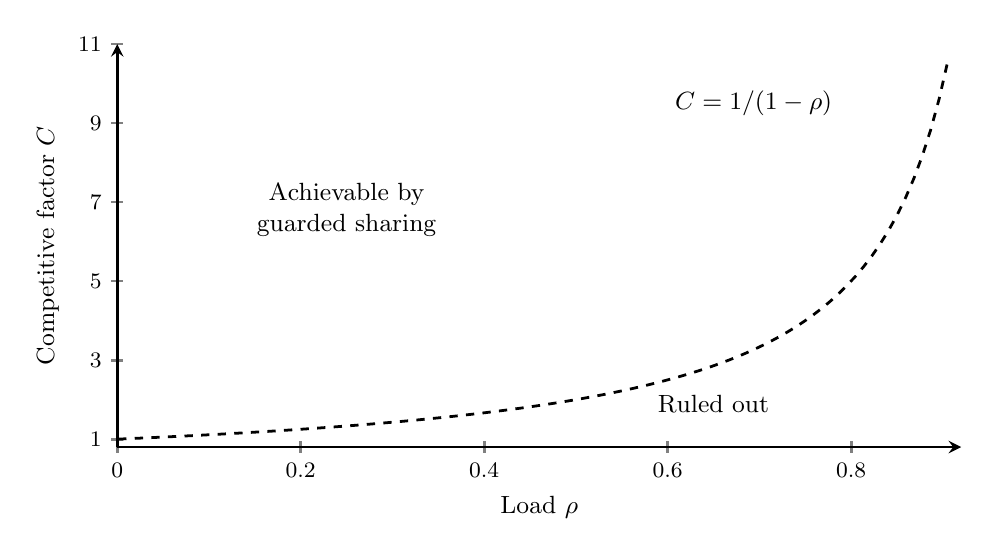
\begin{tikzpicture}
\begin{axis}[
 width=12.3cm,height=6.7cm,
 xmin=0,xmax=.92,ymin=.8,ymax=11,
 xlabel={Load $\rho$},ylabel={Competitive factor $C$},
 xtick={0,.2,.4,.6,.8},ytick={1,3,5,7,9,11},
 axis lines=left,clip=true,
 axis line style={line width=1pt},tick style={line width=1pt},
 tick label style={font=\footnotesize},
 label style={font=\small}]
 \addplot[black,dashed,line width=1pt,domain=.001:.905,samples=100] {1/(1-x)};
 \node[align=center,font=\small] at (axis cs:.25,6.8)
   {Achievable by\\guarded sharing};
 \node[align=center,font=\small] at (axis cs:.65,1.9)
   {Ruled out};
 \node[anchor=east,font=\small] at (axis cs:.79,9.5)
   {$C=1/(1-\rho)$};
\end{axis}
\end{tikzpicture}

\caption{The unit-speed strict boundary. For a fixed load, every competitive factor strictly above the curve is realized by guarded sharing with a job-size-order tail. Factors strictly below it are impossible for eligible policies with that tail guarantee. The curve itself is not classified. The curve is the analytic function $1/(1-\rho)$, not an empirical fit.}\label{fig:phase}
\end{figure}

There are three important exclusions in the converse. A policy that knows the final input horizon need not behave the same on a finite prefix and on an infinite queue, so~\eqref{eq:prefix-opt} cannot be transferred to it without additional work. A message that encodes the future realization likewise invalidates the independence used in~\eqref{eq:cycle-lower}. A bound only in expectation over a policy's randomness does not force pathwise root completion on $E_b$. None is silently included in the theorem.

At $C=1/(1-\rho)$, no finite truncation can satisfy~\eqref{eq:K-choice}: it would require $\rho_K>\rho$. The converse proof therefore stops for a substantive reason. On the positive side, the slower PS comparison would have load one, so its stationary count law cannot be normalized. These two failures do not resolve each other. They identify the equality case as a different question rather than license to replace either strict inequality by a non-strict one.

\section{Finite messages and their encoding}\label{sec:advice}
The strict load boundary now turns a policy-selection problem into an interval-covering problem. The reduction is useful only because the lower side applies to every eligible policy and the upper side gives an actual policy with the stated exact competitive factor. We keep the reduction and the scheduling statements separate.

\subsection{One code covers one logarithmic interval}
Fix an envelope $\theta\in[u,v]$, $1<u<v<\infty$, and write $R=v/u>1$. Suppose a public collection has $M$ policies with finite factors $c_1,\ldots,c_M$, and a valid oracle has inflation at most $\Gamma<\infty$.

If code $m$ is selected at an environment with parameter $\theta$, Theorem~\ref{thm:obstruction} requires $c_m\geq\theta$. The inflation bound requires $c_m\leq\Gamma\theta$. Thus every environment assigned to that code has
\begin{equation}\label{eq:code-interval}
 \theta\in[c_m/\Gamma,c_m].
\end{equation}
A code's actual admissible set may be smaller, or may depend on more than the load. Equation~\eqref{eq:code-interval} is only a necessary containing interval. This suffices for the lower bound, so no monotonicity of a policy's good-tail region is assumed.

\begin{proposition}[Covering lower bound]\label{prop:covering}
Every valid $M$-policy collection on $[u,v]$ has inflation
\begin{equation}\label{eq:cover-lower}
 \Gamma\geq R^{1/M}.
\end{equation}
The lower bound already holds if the service distribution is fixed to one regularly varying finite-mean law and only the Poisson rate varies across the envelope.
\end{proposition}
\begin{proof}
For each $\theta\in[u,v]$, there is an environment at that load. For example, fix any positive regularly varying $B$ with finite mean and choose $\lambda=(1-1/\theta)/\E B$. The valid oracle must select some code for this environment. Therefore the $M$ intervals in~\eqref{eq:code-interval} cover $[u,v]$.

On applying the increasing map $z=\log\theta$, each interval has length $\log\Gamma$. The length of their union is at most $M\log\Gamma$, whether or not they overlap and whether or not they extend outside the target envelope. Covering the interval $[\log u,\log v]$ requires
\[
 \log(v/u)\leq M\log\Gamma.
\]
Exponentiating proves~\eqref{eq:cover-lower}. The construction of an environment at each load used only one service law, proving the last assertion.
\end{proof}

An arbitrary size-aware oracle does not improve this bound. It can change which code is selected, but it cannot make a policy with $c_m<\theta$ have a job-size-order tail at that load. Likewise, within-cycle observations cannot reduce a fixed policy's global worst-case factor in the objective~\eqref{eq:inflation-def}.

\subsection{A collection approaching the lower bound}
Define ideal geometric boundaries
\begin{equation}\label{eq:ideal-boundaries}
 t_j=uR^{j/M},\qquad j=0,\ldots,M.
\end{equation}
For a chosen positive margin $\eps$, use competitive factors and guards
\begin{equation}\label{eq:ideal-guards}
 C_j=(1+\eps)t_j,
 \qquad \delta_j=1/C_j,
 \qquad j=1,\ldots,M.
\end{equation}
The oracle uses the first bin $[t_0,t_1]$ when appropriate, and bin $(t_{j-1},t_j]$ thereafter. The shared-boundary convention makes each selection unambiguous but has no effect on the bounds.

\begin{proposition}[Geometric-bin construction]\label{prop:geometric}
The collection of policies $\GP_{\delta_j}$ from~\eqref{eq:ideal-guards} is valid. Every selected policy satisfies its maximum-flow guarantee on every finite input, regardless of whether the code was appropriate for the environment. Under a correct selection,
\begin{equation}\label{eq:ideal-inflation}
 \frac{c(\GP_{\delta_j})}{\theta}
 \leq(1+\eps)R^{1/M}.
\end{equation}
For a fixed tail index $\alpha>1$ and any integer $p>\alpha$, it also has
\begin{equation}\label{eq:uniform-slack-tail}
 \limsup_{x\to\infty}
 \frac{\Pp(T>x)}{\Fbar((1-\rho)x)}
 \leq H_{\alpha,p}\left(\frac{1+\eps}{\eps}\right)^\alpha.
\end{equation}
\end{proposition}
\begin{proof}
A selected bin has $\theta\leq t_j$, so $C_j\geq(1+\eps)\theta>\theta$. Theorems~\ref{thm:guard-tight} and~\ref{thm:guard-tail} give the exact competitive factor and the tail guarantee. Since $\theta\geq t_{j-1}$, their ratio is at most $(1+\eps)t_j/t_{j-1}=(1+\eps)R^{1/M}$.

For the explicit tail bound, $C_j\geq(1+\eps)\theta$ implies
\[
 \delta_j\leq\frac{1-\rho}{1+\eps},\qquad
 1-\rho-\delta_j\geq\frac\eps{1+\eps}(1-\rho).
\]
Substitute this inequality into~\eqref{eq:guard-tail-gap}. The finite-input guarantee of each policy never used the load and therefore survives an incorrect selection.
\end{proof}

The constants in~\eqref{eq:uniform-slack-tail} are uniform over the selected loads and over slowly varying factors with the same $\alpha$, in the sense of a bound on each law's limsup. This does not exchange a supremum over service laws with the limit in $x$. Regular variation permits arbitrarily late entry into its asymptotic regime, so such an exchange would be a stronger and unsupported statement.

Taking $\eps\downarrow0$ in the inflation bound and combining with Proposition~\ref{prop:covering} establishes the infimum in Theorem~\ref{thm:advice-intro} for ideal real-valued public boundaries. The next subsection shows that finite rational descriptions attain the same infimum. In neither construction is $\eps=0$ used as a valid positive-theorem parameter.

\subsection{Environment messages are not input-advice tapes}\label{sec:message-vs-advice}
The covering theorem uses the cardinality of a fixed policy collection, but its oracle is weaker than the usual advice-on-tape oracle in online algorithms.  In classical advice complexity, the oracle may inspect the realized request sequence and encode information tailored to that sequence~\cite{bocken2009,hromkovic2010,emek2011,komm2011,boyar2016}.  Here the message is chosen from $(\lambda,F)$ before the arrivals and service marks are realized.  Conditional on the selected code, every busy cycle remains random and independent of that choice.  This distinction is indispensable to the obstruction: an oracle that identified the future large-root cycle could encode scheduling information that our model expressly withholds.

There are three separate bit counts.  First, $\lceil\log_2 M\rceil$ bits identify one code when the message is fixed length.  Second, the public collection must describe $M$ policies and their numerical parameters.  Third, an implementation or certifier must determine which public interval contains the environment parameter.  The theorem optimizes the first resource while Sections~\ref{sec:encoding} and the selection analysis account for the latter two.  A short index does not make an irrational boundary or an exponentially large public table free.

This accounting also clarifies nonattainment.  The geometric covering lower bound permits closed intervals of logarithmic length $\log\Gamma$, whereas the positive scheduling theorem requires strict slack $c_m>\theta$.  At a bin's upper endpoint, setting $c_m=\theta$ would invoke the unresolved equality case.  Positive margins therefore approach the covering value but need not attain it.  The word ``infimum'' in Theorem~\ref{thm:advice-intro} records a scheduling boundary, not a numerical artifact of the rational approximation.

A variable-length prefix code would change the objective only after a distribution over environments is specified.  Its expected message length can be finite while its worst-case length is unbounded, and rare environments can select arbitrarily large factors or descriptions.  The fixed-length theorem instead makes a uniform statement on the entire public envelope.  Section~\ref{sec:boundaries} keeps these notions separate rather than converting one into the other by an implicit prior.

\subsection{Rational public codebooks}\label{sec:encoding}
Suppose $u$ and $v$ are rational public inputs. Exact geometric boundaries can be irrational, so they should not be stored as if a finite advice index made their representation free. Fix a positive rational $\zeta$ and an integer grid denominator $D$. Define $q_0=u$, $q_M=v$, and for $1\leq j<M$ set
\begin{equation}\label{eq:rational-boundary}
 q_j=\frac1D\min\left\{n\in\mathbb Z_{\geq0}:
       (n/D)^M\geq u^{M-j}v^j\right\}.
\end{equation}
All comparisons in this definition are rational, hence can be made by integer multiplication and comparison. They do not require evaluating an inexact $M$th root.

For sufficiently large $D$,
\begin{equation}\label{eq:rational-approx}
 t_j\leq q_j\leq(1+\zeta)t_j,
 \qquad q_0<q_1<\cdots<q_M.
\end{equation}
Indeed, $q_j-t_j<1/D$. Every ideal gap is at least $u(R^{1/M}-1)>0$. Taking $1/D$ smaller than that gap and at most $\zeta u$ ensures both properties, including the final gap to the exact endpoint $v$. The inequalities in~\eqref{eq:rational-approx} can themselves be checked without roots by raising positive rational quantities to the $M$th power. An implementation can increase $D$ until the checks succeed.

Use bins with the rational boundaries $q_j$ and factors
\begin{equation}\label{eq:rational-guard}
 \widehat C_j=(1+\eps)q_j,
 \qquad\widehat\delta_j=1/\widehat C_j,
\end{equation}
where $\eps>0$ is rational. The resulting policies have finite rational rate parameters. For a correct selection, $\widehat C_j\geq(1+\eps)\theta$, so the tail bound~\eqref{eq:uniform-slack-tail} is unchanged. Their inflation is at most
\begin{equation}\label{eq:rational-inflation}
 \max_j\frac{\widehat C_j}{q_{j-1}}
 \leq(1+\eps)(1+\zeta)R^{1/M}.
\end{equation}
The leftmost expression is an exact rational certificate for the constructed collection, whether or not one chooses to describe its quality using $\zeta$.

\begin{theorem}[Finite-description infimum]\label{thm:rational-infimum}
For rational $1<u<v$, restricting the positive construction to finite rational boundaries and guards does not change $\Gamma_M^*(u,v)$. In particular, for every $\gamma>R^{1/M}$ there is such a collection with inflation strictly less than $\gamma$ and job-size-order tails throughout the envelope.
\end{theorem}
\begin{proof}
The universal lower bound applies unchanged to finitely described policies. For the upper bound, choose positive rational $\eps$ and $\zeta$ sufficiently small that $(1+\eps)(1+\zeta)R^{1/M}<\gamma$. Choose a finite $D$ satisfying~\eqref{eq:rational-approx}. Equations~\eqref{eq:rational-guard} and~\eqref{eq:rational-inflation}, together with Proposition~\ref{prop:geometric}'s tail argument, give the result.
\end{proof}

For arbitrary real envelope endpoints, the ideal formula still holds. A finite rational public specification can instead use a containing rational envelope. By taking its endpoints sufficiently close, its ratio approaches $v/u$. This is approximation of a fixed public specification, not transmission of an arbitrary real through one message.

\subsection{Encoding cost and selection precision}
Let $L$ bound the binary lengths of the rational numerators and denominators of $u$ and $v$, and let $L_\eps$ do the same for $\eps$. A boundary numerator is at most $\lceil Dv\rceil$, so a stored boundary or guard has $O(L+L_\eps+\log D)$ bits. A list representation of the public collection therefore uses
\begin{equation}\label{eq:table-storage}
 O\bigl(M(L+L_\eps+\log D)\bigr)
\end{equation}
bits, separate from its selected index.

To obtain one boundary in~\eqref{eq:rational-boundary}, binary search among the possible numerators requires $O(L+\log D)$ comparisons. Clearing denominators turns each into a comparison of integers with $O(M(L+\log D))$ bits. Across the table there are $O(M(L+\log D))$ such comparisons; integer powers and products can be computed by ordinary exact arithmetic. This is polynomial in the explicitly represented table dimensions. When $M=2^b$, both the table and its construction may be exponential in the advice budget $b$. No claim of an implicitly succinct policy collection follows from a short index.

The theoretical oracle can classify a real load relative to public thresholds. Exact root arithmetic for the public boundaries does not require the oracle to transmit an exact real load. Strict slack also allows a certified interval of loads to be used instead.

\begin{corollary}[Certified load intervals]\label{cor:load-interval}
Suppose a correct oracle knows an interval $[\ell,h]\subseteq[u,v]$ containing $\theta$, with $h/\ell\leq\kappa_0$. It selects the code for the upper endpoint $h$ in a rational construction with margins $\eps$ and $\zeta$. The tail bound~\eqref{eq:uniform-slack-tail} holds, and the inflation is at most
\begin{equation}\label{eq:interval-inflation}
 (1+\eps)(1+\zeta)R^{1/M}\kappa_0.
\end{equation}
\end{corollary}
\begin{proof}
The selected factor is at least $(1+\eps)h\geq(1+\eps)\theta$, giving the tail bound. Its ratio to $h$ is bounded by~\eqref{eq:rational-inflation}, while $h/\theta\leq h/\ell\leq\kappa_0$. Multiply these inequalities.
\end{proof}

This corollary assumes a certified interval. It is not a learning theorem that obtains such an interval from finitely many observations, and it does not attach an unproved confidence level to an estimated load. An interval extending outside the public envelope needs an enlarged codebook or a separately stated fallback.

\subsection{Advice precision versus the tail-bound constant}
The infimum objective permits the tail constant to become large while the competitive inflation approaches its best value. This feature should be explicit. For an ideal collection write $g=R^{1/M}$ and $s=1+\eps>1$. We have the simultaneous achievable bounds
\begin{equation}\label{eq:constant-tradeoff}
 \Gamma\leq sg,
 \qquad
 \limsup_{x\to\infty}\frac{\Pp(T>x)}{\Fbar((1-\rho)x)}
 \leq H_{\alpha,p}\left(\frac{s}{s-1}\right)^\alpha.
\end{equation}
Rational boundaries add the arbitrarily small inflation multiplier $1+\zeta$ without changing the second inequality.

For example, an analytic target $A>H_{\alpha,p}$ on the displayed upper bound is met whenever
\[
 s\geq\frac{d}{d-1},\qquad d=(A/H_{\alpha,p})^{1/\alpha}>1.
\]
This is a sufficient parameter rule. We do not have a matching lower bound for the best possible tail constant at a given inflation, so the curve in~\eqref{eq:constant-tradeoff} is not asserted to be a Pareto frontier.

The number of fixed-length advice bits can likewise be stated without obscuring equality. To achieve inflation at most $\gamma>1$, a necessary condition is
\begin{equation}\label{eq:bits-necessary}
 2^b\log\gamma\geq\log R.
\end{equation}
The strict inequality is sufficient, since it leaves room for positive $\eps$ and $\zeta$. If equality holds, the infimum statement alone does not prove feasibility at exactly $\gamma$. Treating an infimum as an attained minimum would incorrectly erase the unresolved scheduling boundary.

Together, the lower covering argument, exact factors of guarded sharing, and rational construction prove Theorem~\ref{thm:advice-intro}. The information tradeoff is tied to a specific pair of scheduling guarantees and a specific global observation model. It does not imply the same bit formula for per-job advice, total flow, or a learned policy whose finite-input benchmark is restricted to its training distribution.

\section{What changes with the message or the server}\label{sec:boundaries}
The finite-message theorem concerns a bounded public load envelope, correctly selected advice, and a unit-speed algorithm compared with a unit-speed optimum. We now vary these assumptions one at a time. These consequences use the same capacity argument; they do not combine different observation or resource models into one guarantee.

\subsection{Incorrect advice and unbounded load envelopes}
For a fixed code with guard $\delta$ and exact factor $C=1/\delta$, the deterministic maximum-flow guarantee survives every input and every mistaken belief about the law. Its stationary tail has a strict phase distinction:
\begin{equation}\label{eq:wrong-message-phase}
 \begin{cases}
  \rho<1-1/C: &\text{job-size-order upper bound},\\
  \rho>1-1/C: &\text{integrated-tail lower bound}.
 \end{cases}
\end{equation}
The first line is Theorem~\ref{thm:guard-tail}; the second is Theorem~\ref{thm:obstruction} applied to the same policy. Equality is again not classified. Thus the word ``robust'' can legitimately describe its finite-input maximum-flow certificate, but not a tail guarantee under arbitrary incorrect messages.

\begin{corollary}[No finite collection for all stable loads]\label{cor:finite-all-loads}
No finite public collection of eligible unit-speed policies, each with a finite maximum-flow competitive factor, admits a valid global selection rule for all loads $\rho\in(0,1)$ and regularly varying service laws.
\end{corollary}
\begin{proof}
Let $C_{\max}$ be the largest factor in the finite collection. Choose a load with $\theta(\rho)>C_{\max}$ and fix any regularly varying finite-mean service law. Every possible selected code has factor below $\theta(\rho)$, so Theorem~\ref{thm:obstruction} excludes the required tail for all of them.
\end{proof}

This statement is not a prohibition on finite advice in every environment. Theorem~\ref{thm:rational-infimum} covers any fixed finite envelope. Nor does it rule out a single policy with no finite global competitive factor, such as ordinary PS. The finiteness of the factors is part of the simultaneous guarantee being studied.

\subsection{An unbounded-length code}
A countably infinite family can cover all loads while keeping every individual message finite. Fix rational $u\geq1$. For $\theta\geq u$, choose the integer $j\geq0$ such that
\begin{equation}\label{eq:infinite-bins}
 u2^j\leq\theta<u2^{j+1},
 \qquad C_j=u2^{j+2},\qquad\delta_j=1/C_j.
\end{equation}
Then $2\theta<C_j\leq4\theta$. Taking $u=1$ covers every stable positive load. The policy $\GP_{\delta_j}$ has exact factor $C_j$, inflation at most four, and the tail bound
\begin{equation}\label{eq:variable-tail}
 \limsup_{x\to\infty}\frac{\Pp(T>x)}{\Fbar((1-\rho)x)}
 \leq 2^\alpha H_{\alpha,p}
\end{equation}
for every integer $p>\alpha$. These assertions follow directly from the reservation and tail theorems with multiplicative margin at least two.

One prefix-free encoding is the unary word $1^j0$, of length $j+1$. All its messages are finite, but their lengths have no common finite upper bound. An explicit more compact encoding first writes a self-delimiting representation of the binary length of $j+1$, then the remaining bits of $j+1$. To be precise, put
\[
 m=j+1,\quad \ell=\lfloor\log_2m\rfloor+1,
 \quad k=\lfloor\log_2\ell\rfloor+1.
\]
Write $k-1$ zero bits followed by the $k$-bit binary representation of $\ell$, then the binary representation of $m$ with its initial one removed. The decoder first recovers $\ell$ and then knows exactly how many additional bits to read. No codeword is a prefix of another. Its length is
\begin{equation}\label{eq:delta-length}
 L_j=\ell+2k-2
 \leq\log_2(j+1)+2\log_2(\log_2(j+1)+1)+1.
\end{equation}
The transmitted length is therefore of order $\log\log\theta$, with a further self-delimiting overhead. However, an expanded rational representation of the guard in~\eqref{eq:infinite-bins} needs order $j$ bits. A short code for an exponent is not a constant-size expanded rate parameter or a uniform execution-resource bound.

Fixed worst-case message length and finite expected length are also different. For this prior example only, fix a rational $u>1$ (for instance, $u=2$), and put $\theta_j=u2^j$ with probability $2^{-j-1}$ for $j\geq0$. Every positive-probability support point then has $\theta_j>1$, hence $\rho_j=1-1/\theta_j\in(0,1)$. Moreover, $\theta_j$ lies in bin $j$ of~\eqref{eq:infinite-bins} and is encoded by the unary word $1^j0$, of length $j+1$. The probabilities sum to one, and the expected length is
\[
 \sum_{j\geq0}(j+1)2^{-j-1}=2.
\]
The prior's load support nevertheless approaches one. This is a distribution over queue environments used to count message bits, not a new iid service law obtained by mixing all those queues, and~\eqref{eq:variable-tail} is a conditional statement for each environment.

Finite expected length is not automatic for every prior. For this second prior example also fix a rational $u>1$ (again, $u=2$ is allowed), restrict loads to $\theta_j=u16^j$ for $j\geq0$, and let $(p_j)_{j\geq0}$ be a probability distribution. Every positive-probability support point then has $\theta_j>1$. Requiring inflation at most four, Equation~\eqref{eq:code-interval} shows that one code can serve at most one such value of $j$. Any prefix-free message scheme therefore has expected length at least the entropy $\sum_j p_j\log_2(1/p_j)$. Indeed, prefix-free words of lengths $L_j$ have $\sum_j2^{-L_j}\leq1$, as their corresponding binary cylinders are disjoint. Normalizing these weights and applying nonnegativity of relative entropy gives $\sum_jp_jL_j\geq\sum_jp_j\log_2(1/p_j)$. The inequality for infinite entropy follows by finite truncation. This is a coding consequence of the interval restriction, not an additional tail theorem.

\subsection{An explicitly faster server}
Now change the actual server speed to $\sigma\geq1$, while retaining the \emph{unit-speed} offline comparator in~\eqref{eq:maxflow}. Continue to use $\rho=\lambda\mu<1$ for the nominal unit-speed load; the actual utilization is $\rho/\sigma$. Define guarded sharing at speed $\sigma$ by giving the oldest job rate $\delta$ plus its equal share of $\sigma-\delta$, for $0<\delta<\sigma$.

The finite-input prefix argument gives
\begin{equation}\label{eq:fast-competitive}
 \MF_{\GP_{\sigma,\delta}}(I)\leq\frac{\OPT(I)}\delta.
\end{equation}
To justify the comparison, the faster work-conserving workload is no larger than the unit-speed workload on the same input. A prefix therefore has at most $\OPT(I)$ remaining work at its release time, and it receives at least rate $\delta$ until completion. The slower-PS comparison now has speed $r=\sigma-\delta$. If $\rho<r$, Lemma~\ref{lem:conditional-ps} and its integration still apply with that value of $r$.

The obstruction changes by the same amount of capacity.

\begin{proposition}[Speed-explicit obstruction]\label{prop:speed-obstruction}
Let an eligible policy run at speed $\sigma\geq1$ with competitive factor $C$ relative to the unit-speed maximum-flow optimum. For a nominally stable regularly varying environment with $0<\rho<1$, if
\begin{equation}\label{eq:fast-obstruction}
 C<\frac1{\sigma-\rho},
\end{equation}
then its stationary response satisfies the integrated-tail lower bound
\[
 \liminf_{x\to\infty}\frac{\Pp(T>x)}{x\Fbar(x)}>0.
\]
\end{proposition}
\begin{proof}
A feasible factor is at least $1/\sigma$, by considering a single job. Under~\eqref{eq:fast-obstruction}, choose $K$ with $\rho_K>\sigma-1/C$, then choose
\[
 C<\kappa<\frac1{\sigma-\rho_K},
 \qquad\Delta=1-\kappa(\sigma-\rho_K)>0.
\]
Use the same positive constants $e$, $\eta$, and $c_0$ as in~\eqref{eq:epsilon-choice}--\eqref{eq:eta-choice} with this $\Delta$. The finite prefix is still compared against the unit-speed optimum. Since $\rho<1$, its workload bound~\eqref{eq:prefix-opt} remains valid, and the root must complete before $H=\kappa b$.

The actual queue cannot empty by $H$, because $b+A_K(t)-\sigma t\geq(\Delta-e)b>0$ for $t\leq H$. After the root completes, subsequent bounded jobs have received at most $\sigma H-b$ service. Their remaining work is at least
\[
 A_K(H)-(\sigma H-b)\geq(\Delta-e)b.
\]
The same size cap and recent-arrival subtraction leave at least $c_0b$ old unfinished jobs. Finally the actual-speed busy-cycle offspring mean is $\lambda\mu/\sigma=\rho/\sigma$, so its expected arrival count is $1/(1-\rho/\sigma)$. The proof of Theorem~\ref{thm:obstruction} applies with this cycle factor, giving a positive lower constant.
\end{proof}

\begin{theorem}[Zero advice with speed augmentation]\label{thm:zero-advice-speed}
Fix $\eps>0$. At actual speed $1+\eps$, a single nonclairvoyant eligible policy has a maximum-flow factor $1/\eps$ relative to the unit-speed optimum and a job-size-order stationary tail for every nominal load $\rho\in(0,1)$ and every regularly varying service law with finite mean. No smaller uniform factor is possible for this simultaneous guarantee within the eligible class.
\end{theorem}
\begin{proof}
Use $\delta=\eps$ and residual PS speed $r=1$. Equation~\eqref{eq:fast-competitive} gives factor at most $1/\eps$. The PS comparison is stable at every $\rho<1$, and Theorem~\ref{thm:guard-tail}'s integration gives the tail guarantee. In fact, the scaled tail upper constant from that proof is at most $H_{\alpha,p}$.

Conversely, if a fixed policy had uniform factor $C<1/\eps$, choose $\rho<1$ sufficiently close to one that $C<1/(1+\eps-\rho)$. Proposition~\ref{prop:speed-obstruction} would exclude its required tail at that load. Therefore a smaller uniform factor is impossible, and the construction attains $1/\eps$.
\end{proof}

This theorem does not remove the need for advice in the unit-speed theorem by giving its algorithm an unstated advantage. It changes an explicit resource. Its equality $C=1/\eps$ is uniform over loads approaching one; at every fixed $\rho<1$, it lies strictly above $1/(1+\eps-\rho)$. Hence it does not resolve the fixed-load equality case left open earlier.

\section{Exact finite consequences and negative controls}\label{sec:finite}
The proofs above contain limiting and stationary arguments that cannot be established by bounded execution. We nevertheless check the finite scheduling rules and several algebraic consequences exactly. The purpose is to expose implementation mistakes in the proposed policy, benchmark, or encoding, not to turn a count of generated instances into evidence of an asymptotic tail law.

\subsection{A separate finite deadline oracle}
The main finite campaign uses all multisets of one through five jobs from the six release/size pairs with release in $\{0,1,2\}$ and size in $\{1,2\}$. There are
\[
 \sum_{n=1}^5\binom{n+5}{5}=461
\]
such inputs. For each, an exhaustive integer-slot oracle searches relative deadlines from the largest size upward. Its states record the integer time and the remaining integer processing requirements. At each slot it tries every available unfinished job, as well as deliberate idling. A state is infeasible when an unfinished job has reached its relative deadline.

This oracle does not use the workload identity to determine its answer. Its returned optimum agreed with FCFS on all 461 inputs. It visited 188,745 states across the searches. It is an oracle for the stated slotted model; the general continuous-time identity is supplied by Lemma~\ref{lem:workload}, not inferred from this agreement.

For each input we simulated guards $1/4$, $1/2$, and $3/4$, giving 1,383 policy comparisons. Arrival times, rates, residuals, and completions were rational throughout. A trace checker recomputed capacity, conservation, active intervals, work conservation, prefix reservation, and attained-service domination over PS at speed $1-\delta$. Separately, a reference implementation reconstructed policy breakpoints without consuming production segments; it matched 2,856 completion vectors from 714 rational inputs under four speed--guard configurations. Three mutated rules---youngest protection, an extra sharing denominator, and an omitted reserve---produced different vectors. All finite maximum-flow comparisons satisfied Theorem~\ref{thm:guard-competitive}. The guarded integer schedules needed at most 20 bits per completion numerator or denominator.

The rate selector uses only the active set and oldest-job order. Sizes are ground truth for detecting completion events, but are not consulted when selecting rates; this is the relevant nonclairvoyance distinction.

\subsection{Controls that distinguish the claimed invariant}
Replacing the oldest-job reservation by a youngest-job reservation produces a valid work-conserving schedule but invalidates the prefix proof. On the 49-job control instance with guard $1/2$, offline maximum flow is one. Correct guarded sharing has maximum flow approximately $1.735241$, while the youngest-reservation control has maximum flow $13/4>2$. The prefix-reservation checker rejects the latter. A separate corruption that adds one to every reported completion is also rejected by the service/active-interval checks.

These controls test different failures. The youngest-job control preserves ordinary feasibility and capacity, so a checker that only verifies served work would miss the scheduling defect. The completion corruption tests the trace certificate rather than the rate choice. Neither control is a hostile workload against an external system; both are finite synthetic mathematical inputs.

Boundary tests additionally cover empty and singleton inputs, coincident arrivals and completions, zero and full reservation endpoints in the finite simulator, time translation, common rational scaling of releases and sizes, invalid inputs, malformed traces, and speed-augmented comparisons. Zero reservation is tested as ordinary PS, not asserted to have the guarded policy's finite factor. Full reservation is tested as FCFS, not assigned the positive theorem's strictly positive residual PS capacity.

\subsection{A claim-to-check boundary}\label{sec:finite-boundary}
The campaign is organized around falsifiable interfaces rather than one ``all tests passed'' flag. Table~\ref{tab:check-boundary} states what each executable layer can reject and what remains mathematical. FCFS/oracle and production/reference agreement exercise separately written paths, while emitted traces are recomputed rather than trusted; none of these finite agreements proves the corresponding all-input lemma.

\begin{table}[t]
\centering
\small
\caption{Executable checks and their proof boundary.  ``All'' in the last column refers to the theorem's quantified domain, not to the enumerated sample.}\label{tab:check-boundary}
\begin{tabular}{@{}L{0.22\textwidth}L{0.34\textwidth}L{0.34\textwidth}@{}}
\toprule
Layer & What the executable evidence can reject & What still requires the written proof\\
\midrule
Deadline oracle & Incorrect finite optimum or FCFS implementation on the enumerated integer instances & Workload optimality for arbitrary real releases, sizes, and input lengths\\
Trace certificate & Capacity, conservation, active-interval, work-conservation, and prefix-reservation violations & Exact factor for all finite inputs and the limiting tightness construction\\
PS comparison & Failure of attained-service domination on checked rational traces & Stationary residual law and pathwise domination for all sample paths\\
Algebra checks & Incorrect count recurrence, Eulerian coefficients, moments, or rational bin inequalities & Infinite recurrences, invariant-measure identification, and the covering infimum\\
Negative controls & A checker too weak to distinguish feasibility from the claimed invariant & Absence of every possible implementation or proof error\\
\bottomrule
\end{tabular}
\end{table}

The controls were chosen to preserve one layer while breaking another.  Youngest-job reservation remains feasible and work conserving but violates the prefix invariant.  A shifted completion report can preserve the rate rule but violates service accounting.  An ordinary geometric count is a legitimate PS count law in the system without a permanent customer, yet it fails the balance recurrence for the comparison system actually used.  These are more discriminating than malformed inputs that every parser would reject.

Reproduction separates exact outputs from symbolic constants.  A second layer of exact arithmetic audits 16 interfaces: count convolutions, conditional share inequalities, Pareto identities, covers, regenerative ratios, and the strict capacity deficit.  It checks 71 strict-gap choices and 71 equality substitutions; equality correctly leaves the current method without a positive interval.  Wrong count laws, a missing tag in a denominator, and time weighting in place of arrival weighting are rejected.  These diagnostics expose algebra or quantifier errors, but cannot prove invariant measures, a uniform law of large numbers, or transfer under regular variation.  No pass condition observes a desired tail; the limit claims remain written proof obligations.

\subsection{Finite encodings and analytic examples}
Table~\ref{tab:advice} gives an exact rational construction on $\theta\in[2,512]$ with margin $\eps=1/8$ and grid denominator 1024. There are 31 public entries across the five separately constructed codebooks. Exact endpoint and midpoint selections, inequality checks, and out-of-envelope rejections were performed. The table's infimum column comes from Theorem~\ref{thm:advice-intro}; the constructed bound is the exact maximum $\widehat C_j/q_{j-1}$ for the delivered rational entries.

\begin{table}[t]
\centering
\caption{Finite codebooks on $[2,512]$. The first bound is an analytic infimum, not necessarily attained. The construction uses positive margin $1/8$ and finite rational endpoints.}\label{tab:advice}
\begin{tabular}{rrrr}
\toprule
Bits $b$ & Policies $2^b$ & Infimum & Constructed bound\\
\midrule
0 & 1 & $256$ & $288$\\
1 & 2 & $16$ & $18$\\
2 & 4 & $4$ & $9/2$\\
3 & 8 & $2$ & $9/4$\\
4 & 16 & $\sqrt{2}$ & $26073/16384$\\
\bottomrule
\end{tabular}
\end{table}

The artifact also verifies 256 instances of the permanent-customer count-balance identity, 32 moment inequalities, and the Eulerian polynomial identity through order eight. A plain geometric count, incorrectly substituted for the permanent-customer count, fails the balance check. These finite identities help detect a missing factor $n+1$; the stationary-law proof still requires the residual-state argument of Lemma~\ref{lem:ps-invariant}.

Table~\ref{tab:tightness} evaluates six finite members of the deterministic tightness family. All have offline maximum flow one. The displayed responses are rounded for reading; the corresponding fractions are retained in the artifact. Their rational completion representations use at most 457 bits. No convergence rate or limiting supremum is inferred from these six values; Theorem~\ref{thm:guard-tight} proves the limit using a fixed-$\eta$ bound followed by $\eta\downarrow0$.

\begin{table}[t]
\centering
\caption{Finite root responses in the tightness family. The last column is the analytically proved competitive supremum. Finite values below it are not estimates of a stationary tail.}\label{tab:tightness}
\begin{tabular}{rrrrr}
\toprule
Guard & $1/h$ & Jobs & Root response & Supremum\\
\midrule
$1/4$ & 8 & 41 & 2.448618 & 4\\
$1/4$ & 16 & 81 & 2.914706 & 4\\
$1/2$ & 4 & 13 & 1.403571 & 2\\
$1/2$ & 8 & 25 & 1.592010 & 2\\
$1/2$ & 16 & 49 & 1.735241 & 2\\
$1/2$ & 32 & 97 & 1.834847 & 2\\
\bottomrule
\end{tabular}
\end{table}

All finite checks use one worker and standard-library exact arithmetic. The largest illustrated instance has 97 jobs. There is no random seed because no random sampling is performed. In particular, there is no finite service-size cutoff used to estimate a heavy-tail exponent, no warm-up heuristic for a stationary simulation, and no empirical production-latency claim. The truncation by $K$ in the converse is a fixed analytic device inside a proof; it is not a simulated replacement of the service distribution.

\section{Consequences and limits}\label{sec:discussion}
The joint requirement identifies a specific role for global advice. At a fixed load, $1/(1-\rho)$ is the infimum maximum-flow factor compatible with the proved tail-order objective. A finite message chooses among finitely many such factors, and the best inflation over a bounded load envelope is governed by logarithmic covering. The geometric bins are not themselves a new scheduling principle. They become meaningful because a universal capacity obstruction and a nonclairvoyant construction meet on opposite sides of the same strict boundary.

\subsection{What the boundary says about information}
The advice message supplies coarse environmental information, not clairvoyance about jobs.  Once a code is selected, guarded sharing uses only release order and the active population.  Its deterministic certificate is valid on every finite input, including inputs that have zero probability under the advertised environment.  Correct advice is used only to place the residual PS rate above the stochastic load.  This division of labor differs from a predictor that supplies per-job sizes, ranks, or future arrivals, and from an online-advice tape constructed after seeing the realized sequence.

The lower bound shows that this coarse information cannot compensate for a factor below the load boundary.  It permits the competing policy to observe sizes of arrived jobs, to maintain arbitrary within-cycle history, and to depend on the selected environment code.  What it forbids is future realization information and cross-cycle state outside the declared reset.  Thus the obstruction is not caused by nonclairvoyance of the positive rule.  It is caused by the amount of capacity a finite-prefix maximum-flow deadline forces onto a large root.

At the covering infimum, $\log\Gamma_M^*(u,v)=\log(v/u)/M$: the covered coordinate is $\log\theta$, not $\log M$.  This does not make all distributional information one-dimensional.  The tail constant in Theorem~\ref{thm:guard-tail} also depends on the regular-variation index through the analysis, and finer objectives could depend on the slowly varying factor or on the entire law.  Our result says that, for the stated order objective and construction, one load bin suffices; it does not say that load is a sufficient statistic for every scheduling goal.

\subsection{Relation to richer scheduling information}
Service-time information can be used in many other ways.  Two-class and rank-based policies interpolate between blind and fully size-aware scheduling~\cite{chen2021,scully2018soap}; Gittins and related indices optimize stochastic mean objectives under distributional information~\cite{gittins2011,aalto2009,scully2020gittins}; and large-deviation priority rules optimize different rare-event criteria~\cite{stolyar2001}.  These mechanisms may improve constants or objectives that guarded sharing does not target.  None directly supplies the exact maximum-flow certificate proved by the oldest-job reserve, because that certificate protects every released prefix rather than an average or asymptotic state.

Conversely, the reserve is not proposed as universally efficient.  It deliberately spends a fixed rate on the oldest job even when a size-aware rule would prefer another job.  The point is analytical compatibility: the reserve gives a pathwise prefix deadline, while the shared rate gives every job a stable comparison queue.  Any alternative policy that improves one side must still expose an interface strong enough to prove the other.  A promising route is to replace the constant reserve by a state-dependent certificate whose cumulative service to every prefix can be lower-bounded, but the tail comparison would then have to tolerate a time-varying residual capacity.

\subsection{Which hypotheses are structural}
Several distinctions limit how the theorem should be used. The deterministic guarantee concerns the maximum response, not total response or a competitive fairness criterion. The stochastic guarantee concerns a typical arrival in an M/G/1 queue, not worst-case release sequences. Its service laws have regularly varying tails with index below $-1$, and the policy class has an empty-state reset and no future-horizon input. A fixed code remains maximum-flow competitive under incorrect advice, but it need not retain the tail guarantee. Removing any of these restrictions is a separate theorem obligation.

The Poisson assumption is more than a convenient arrival rate.  It supplies the stationary-arrival sampling and invariant PS environment used by the upper bound, and the independent future marked process used by the lower bound.  Renewal arrivals may preserve the fluid event but change what an arrival sees and how a permanent tagged customer is initialized.  A non-Poisson extension therefore needs a Palm version of both halves, not only a renewal strong law.

The single-server assumption is equally structural.  On parallel servers, unfinished work no longer determines maximum flow: placement and fragmentation matter, and an oldest job may be blocked behind work assigned elsewhere.  Multiserver SRPT and Gittins results show that even stochastic response analysis requires new coupling ideas~\cite{grosof2018,scully2020gittins,hong2024}.  An advice boundary in that setting would need a new adversarial benchmark and likely more than one scalar environmental coordinate.  The present formula $(v/u)^{1/M}$ should not be extrapolated to it.

The construction deliberately uses a stronger tail-analysis comparison than its rate rule needs to implement. Every job receives enough shared service to be compared with a stable PS queue, while an oldest-job reservation protects all prefixes. The permanent-customer proof shows why a high conditional response moment can be useful even when the corresponding service moment is infinite: the moment is first taken over a light-tailed customer count, conditional on service size, and only then integrated through a truncated moment. Interchanging these steps would demand a nonexistent high service moment and lose the regularly varying cases of interest.

The converse has a complementary structure. It counts old bounded jobs left after a forced large-job completion. It does not equate backlog volume with queue length, and it does not count overlapping large-job events throughout a stationary history. Restricting the trigger to one root per regenerative cycle makes the reward integrable and the conversion to a Palm arrival probability explicit. This is the step that yields the factor $x$ separating the two tail orders.

\subsection{Open analytical boundaries}
The equality boundary $C=1/(1-\rho)$ remains unclassified. Both present proofs lose their strict capacity margin there, for different reasons. The exact finite-advice statement is therefore an infimum, including at public bin endpoints. Resolving equality may require a policy whose spare capacity vanishes with state or age, together with a tail proof that does not compare against a strictly stable slower queue. A converse would need to extract an order-$x$ cohort without choosing a truncation whose load exceeds $1-1/C$, which is impossible at equality by monotone convergence. Neither direction follows by taking a limit in the existing theorems.

An optimal leading tail constant is also not determined. The supplied upper constants establish order and quantify sufficient slack, but the permanent-customer enlargement and Markov inequality are not expected to be sharp. Classical PS asymptotics suggest that stronger distributional assumptions could improve constants~\cite{yashkov1987,zwartboxma2000,borst2006}. A matching lower constant for the joint objective would require optimizing over all eligible policies, not only analyzing guarded sharing.

Randomization is another genuine boundary.  A pathwise competitive factor for every random seed would reduce to the deterministic theorem seed by seed.  An expected factor, or a high-probability factor against an oblivious adversary, has different quantifiers and does not force the large root to finish on each fluid-event path.  Establishing a randomized analogue would require stating the adversary's access to the seed and replacing the deterministic cohort argument accordingly.

There is a further difference between global advice and a learned scheduler. A message may be selected from a certified load interval, but this work does not infer such an interval from traffic. No finite-sample estimation or predictor-robustness statement is implicit in the oracle model. Learning-augmented scheduling results emphasize consistency, robustness, or fairness under explicit prediction errors~\cite{purohit2018,mitzenmacher2022,li2025,cosson2026}; those guarantees cannot be obtained by relabeling a certified interval as a learned estimate. A statistically grounded extension would need a sampling protocol, confidence event, nonstationarity model, and fallback analysis when the interval misses the true load.

Similarly, an unbounded-length code can have finite expected length under a specified prior while still requiring arbitrarily large expanded parameters. Those are distinct resource notions. The speed-augmentation theorem changes actual service capacity and keeps the unit-speed comparator explicit; it is not an alternative interpretation of the unit-speed advice result.

\subsection{Discriminating next steps}\label{sec:next-steps}
The unresolved directions admit concrete tests that distinguish a real extension from a reformulation.  For the equality case, a positive result must exhibit a policy with exact factor $\theta(\rho)$ and prove a tail bound without a strictly stable constant-rate PS comparison.  A natural candidate would let the oldest-job reserve approach $1/\theta$ only when its prefix certificate is endangered, returning more capacity to sharing at other times.  Such a rule is useful only if one can prove both a cumulative prefix-service inequality and a stochastic comparison whose effective spare capacity does not vanish on the trajectories that dominate the tail.  Conversely, an equality lower bound must replace the strict truncation inequality~\eqref{eq:K-choice}; merely taking $K\to\infty$ in the present constants sends the delayed-cohort margin to zero.

For non-Poisson input, three replacements are independently necessary.  A renewal or mixing process must supply a growing-window fluid event after a cycle root; the root and its future input must be coupled in the correct Palm law; and the positive proof needs either an invariant residual description or another conditional response bound for the comparison queue.  Verifying only the first item would leave both the typical-arrival interpretation and the permanent-customer construction unsupported.  A useful first target is a renewal process with a nonlattice interarrival law and finite variance, where regenerative cycles remain available but PASTA does not.

For parallel servers, the first obligation is deterministic rather than asymptotic.  One must identify the correct finite-input maximum-flow optimum when migration, splitting, and preemption are specified.  Total workload divided by total capacity is only a lower bound because jobs cannot necessarily use all servers simultaneously.  An exact small oracle could expose whether an oldest-job guard on one server, a global fractional reserve, or a migratory rule has any bounded ratio before a heavy-tail analysis is attempted.  Only after that benchmark is settled would a multiserver analogue of the delayed-cohort obstruction be meaningful.

\subsection{Evidence boundary}
The exact finite checks exercise the algebraic service accounting, the finite workload oracle, codebook construction, balance recurrences, and selected boundary cases.  They are useful because they expose implementation mistakes such as counting capped work as bounded jobs or using the ordinary geometric count for the permanent-customer system.  They do not prove regular variation, convergence of a stochastic process, or any theorem quantified over all finite inputs.  Those claims rest on the written arguments.

The mathematical conclusion is therefore confined but joint: under one declared observation model, the same policy has both guarantees, and a lower bound applies to every policy in the comparison class. The proof does not classify equality, optimize the leading constant, estimate advice from data, or establish a multiserver analogue. Those limitations mark concrete next problems rather than exceptions hidden inside the theorem statement.

\bibliographystyle{plain}
\bibliography{references}
\end{document}
